\documentclass[]{report}

\usepackage{subfig}
\usepackage{tikz}
\usepackage{pgfplots}
\usepackage{pgfplotstable}
\usepackage{booktabs}

% Title Page
\title{What I did at Fraunhofer IGD}
\author{Seyedmorteza Mostajabodaveh}


\begin{document}
\maketitle

\begin{abstract}
In November 2014, I moved to Darmstadt to work in Fraunhofer IGD and do my master thesis. In this report, I will present the tasks which I have done beside my master thesis at Fraunhofer IGD as Hiwi. Additionally, my supervisor Andreas Dietrich (TODO:AndreasEmailAddress) which was working at Fraunhofer IGD before was directing me toward these tasks. You can contact him for more information.
\end{abstract}

\begin{figure}[!ht]
	\subfloat{%
		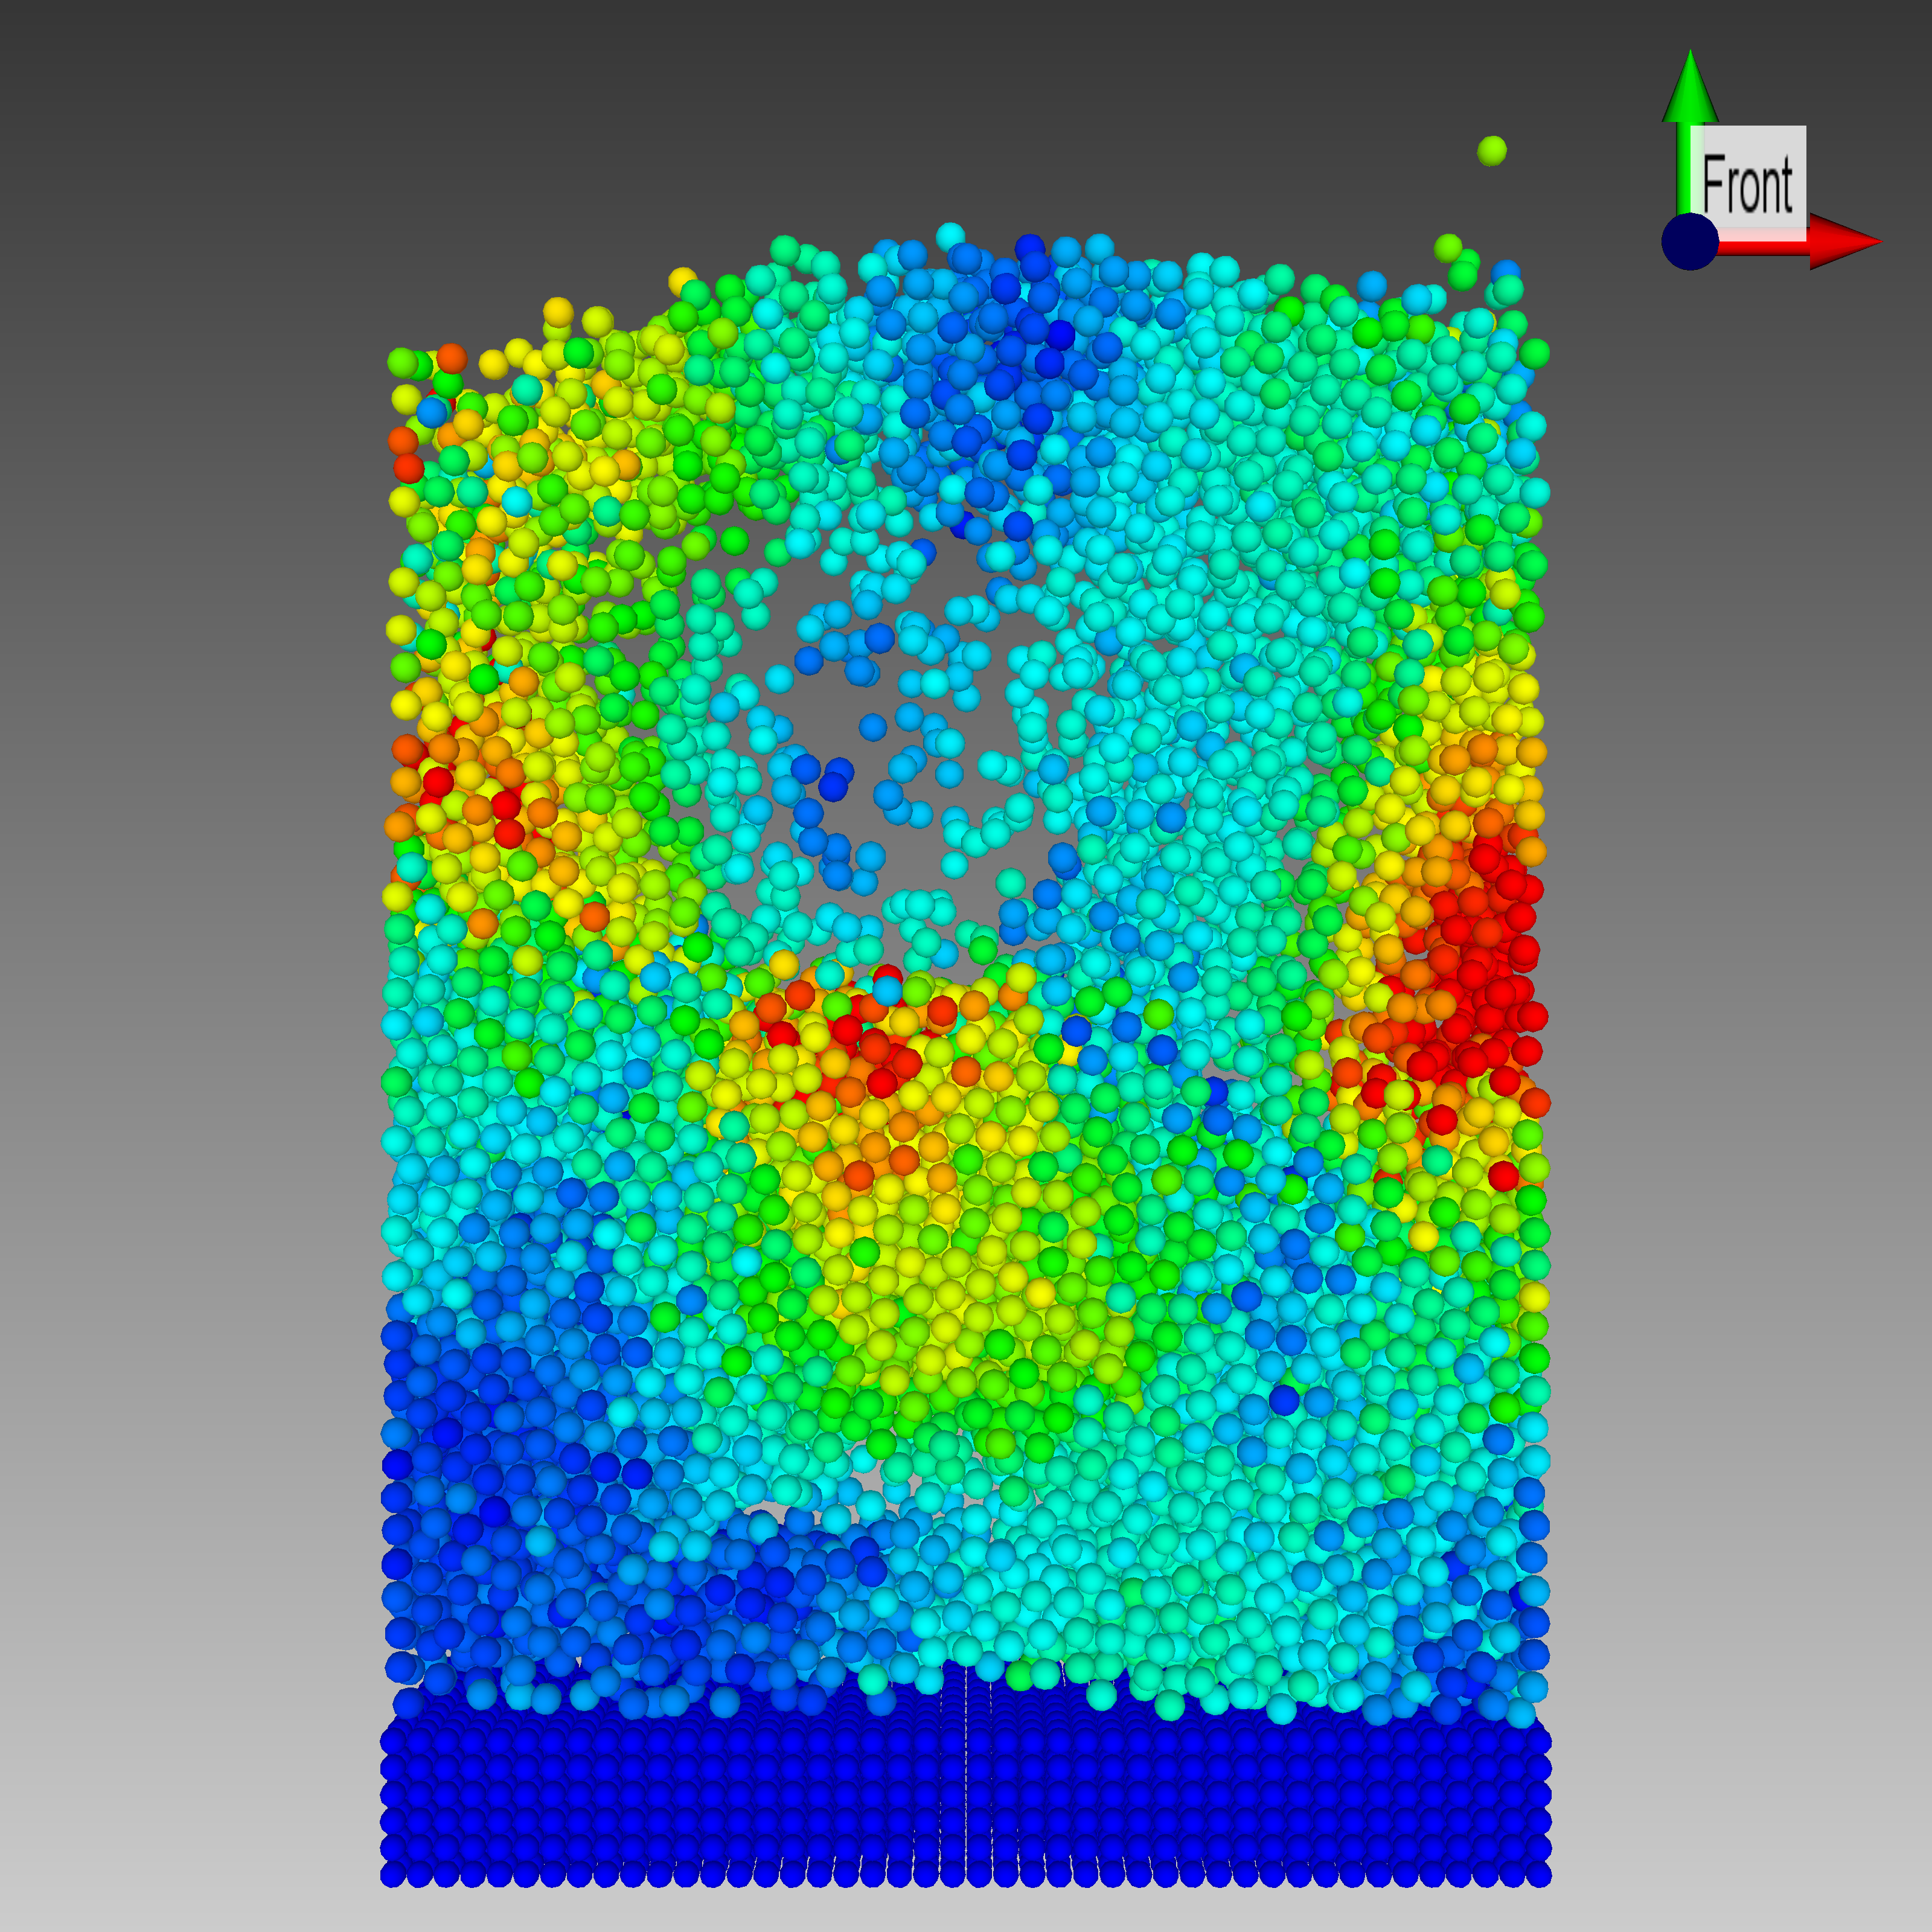
\includegraphics[width=0.2\textwidth]{./figs/particles/new/1.png}
	}
	\hfill
	\subfloat{%
		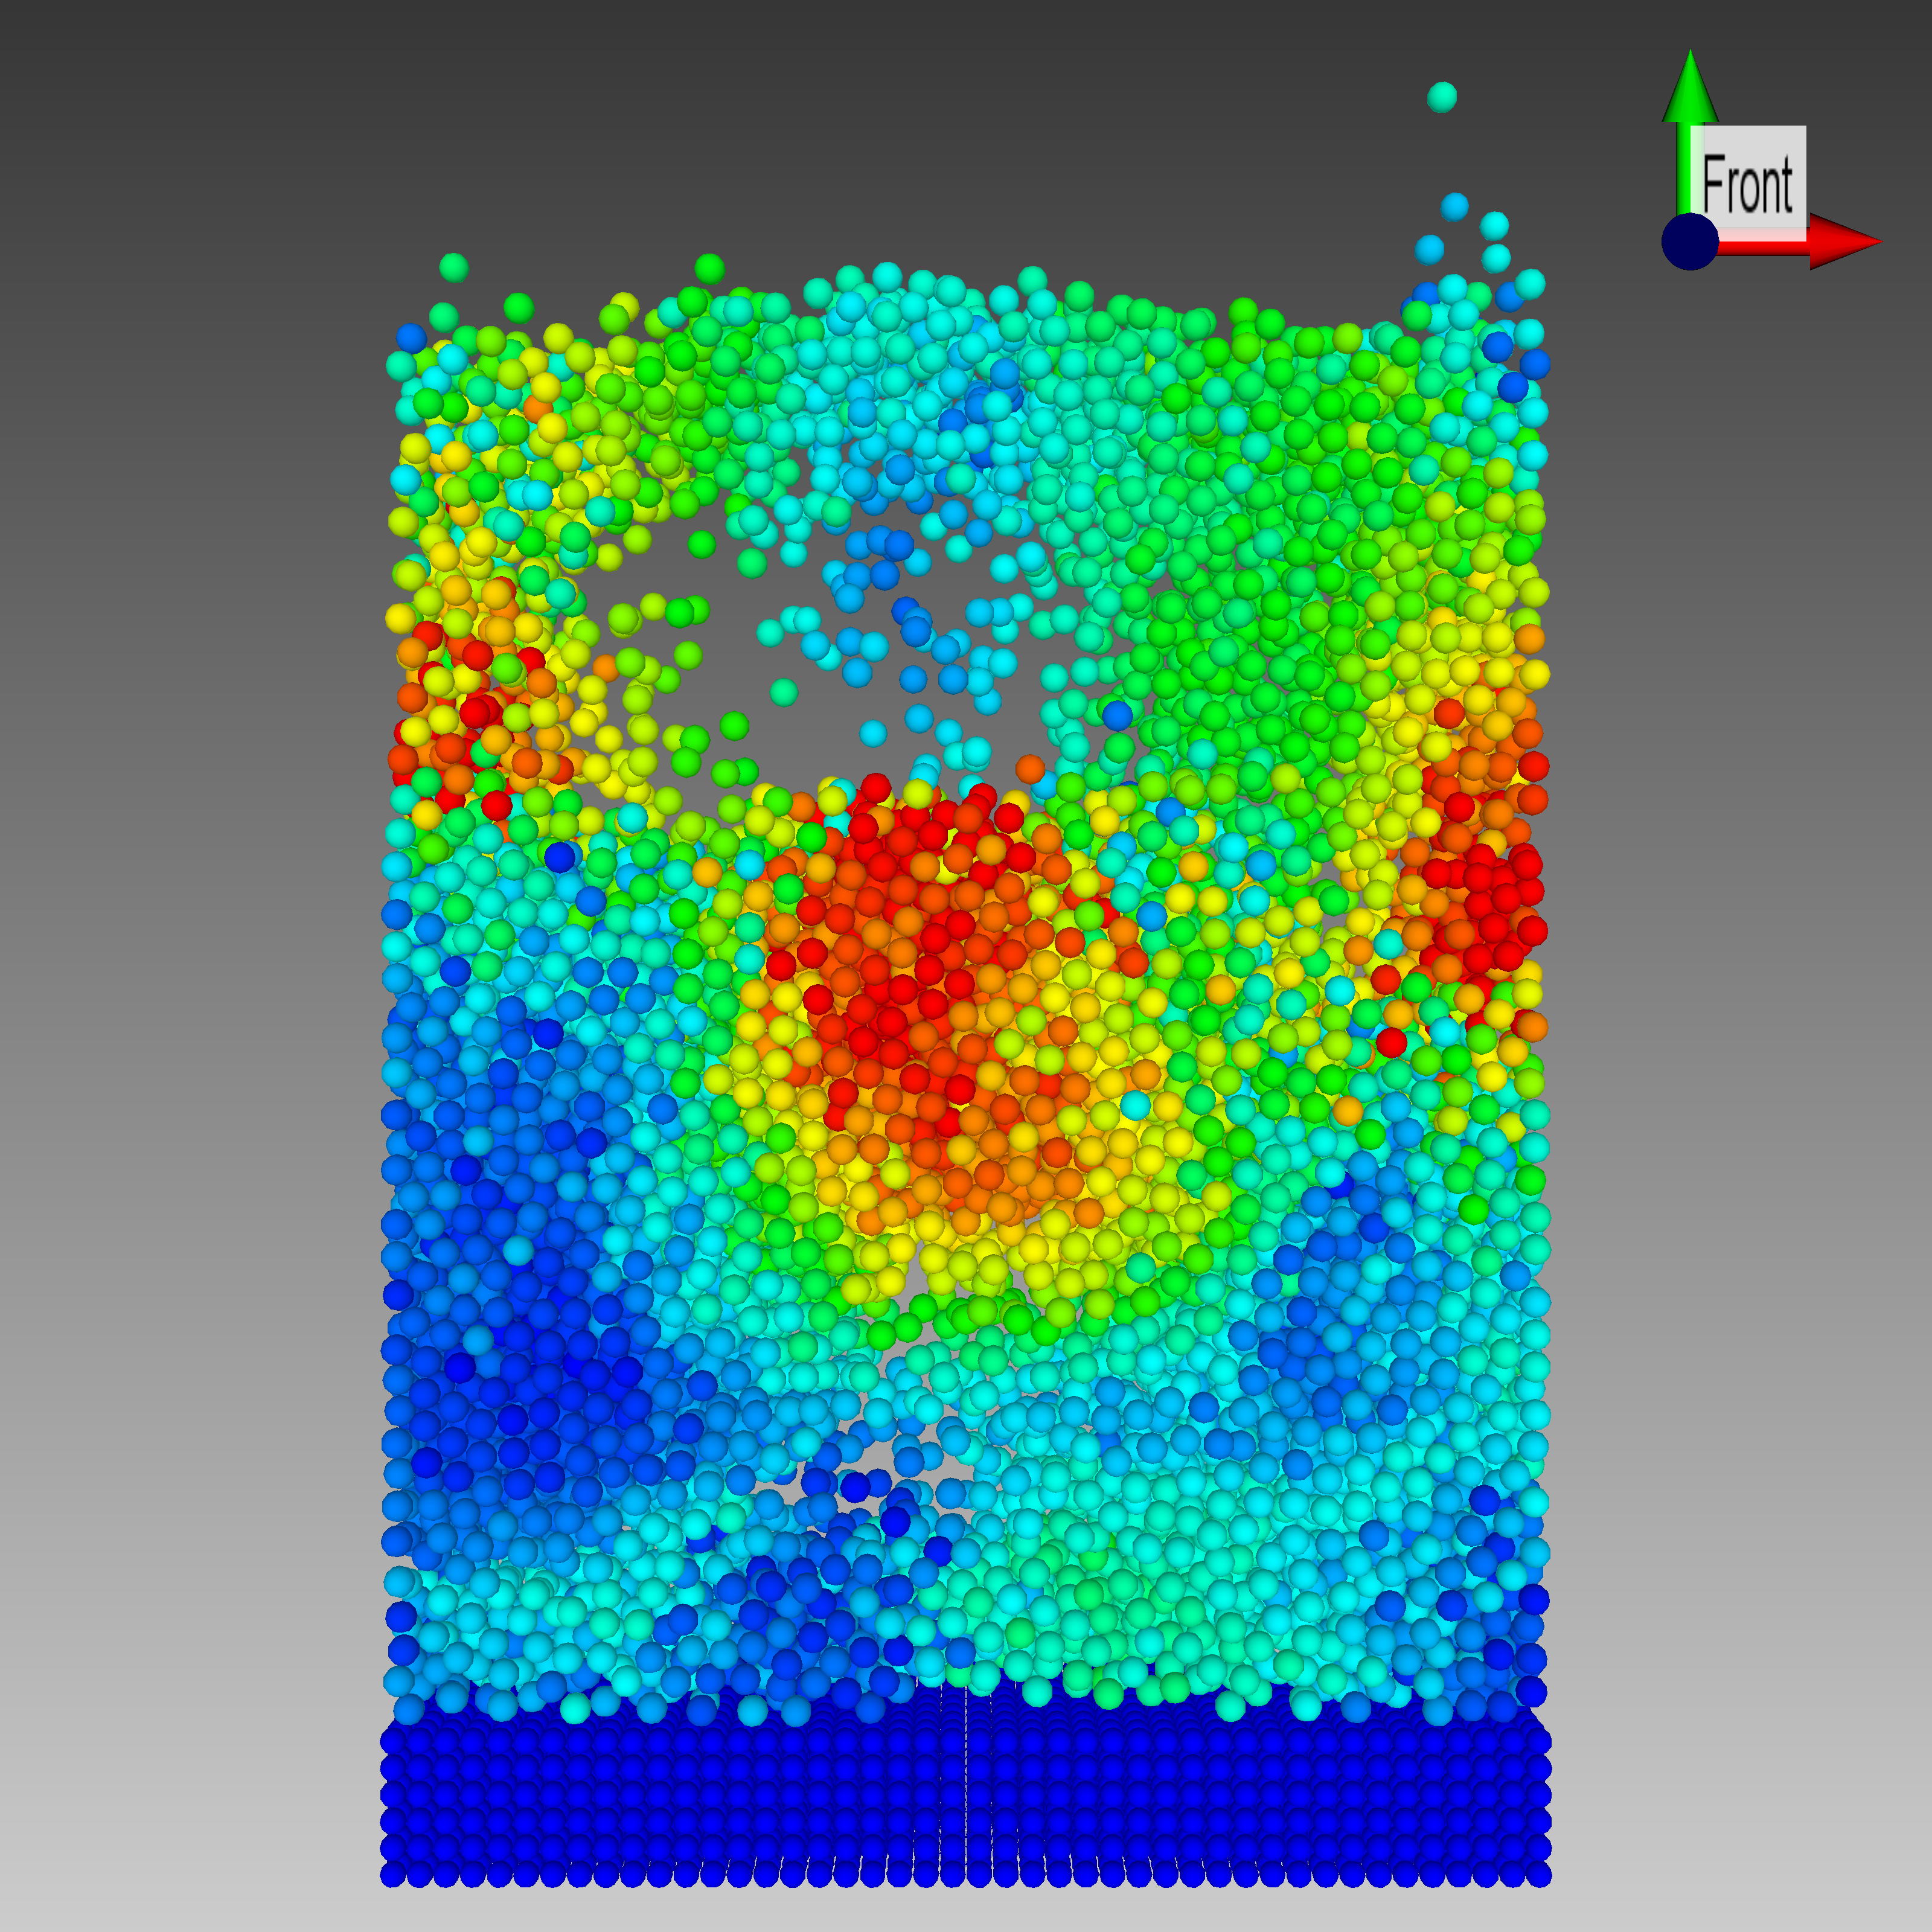
\includegraphics[width=0.2\textwidth]{./figs/particles/new/2.png}
	}
	\hfill
	\subfloat{%
		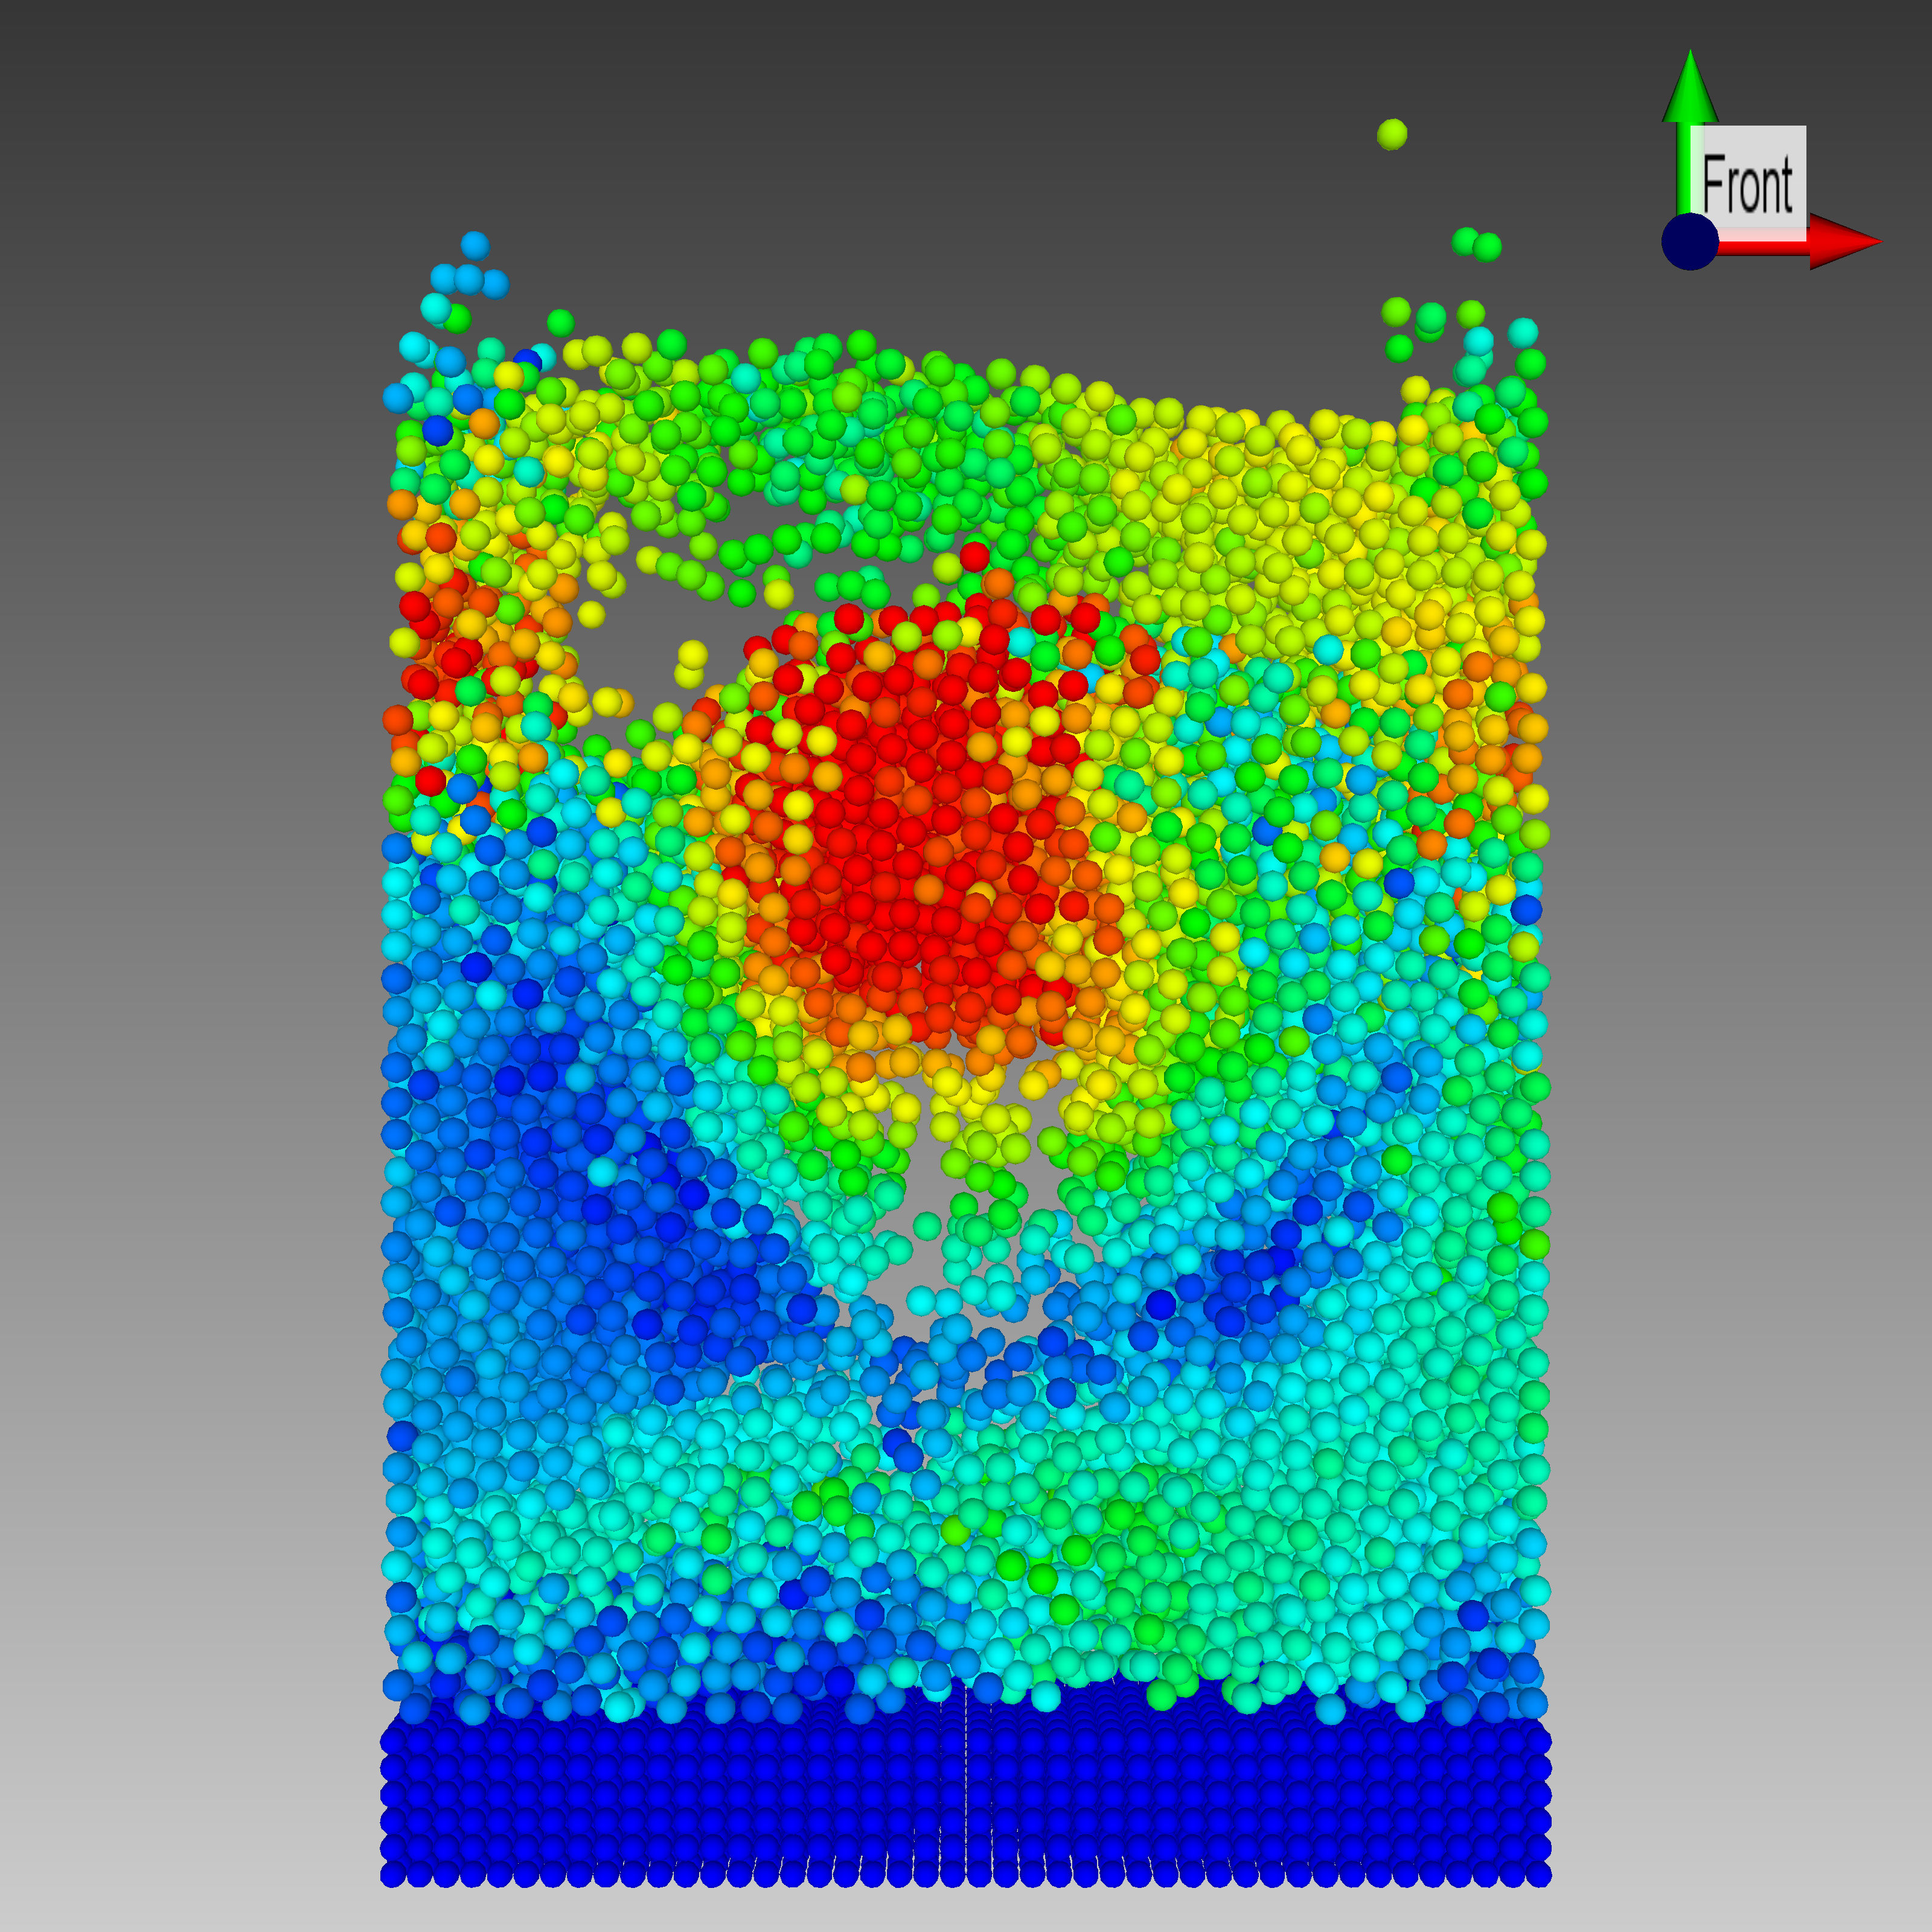
\includegraphics[width=0.2\textwidth]{./figs/particles/new/3.png}
	}
	\hfill
	\subfloat{%
		\includegraphics[width=0.2\textwidth]{./figs/particles/new/4.png}
	}
	\hfill
	\subfloat{%
		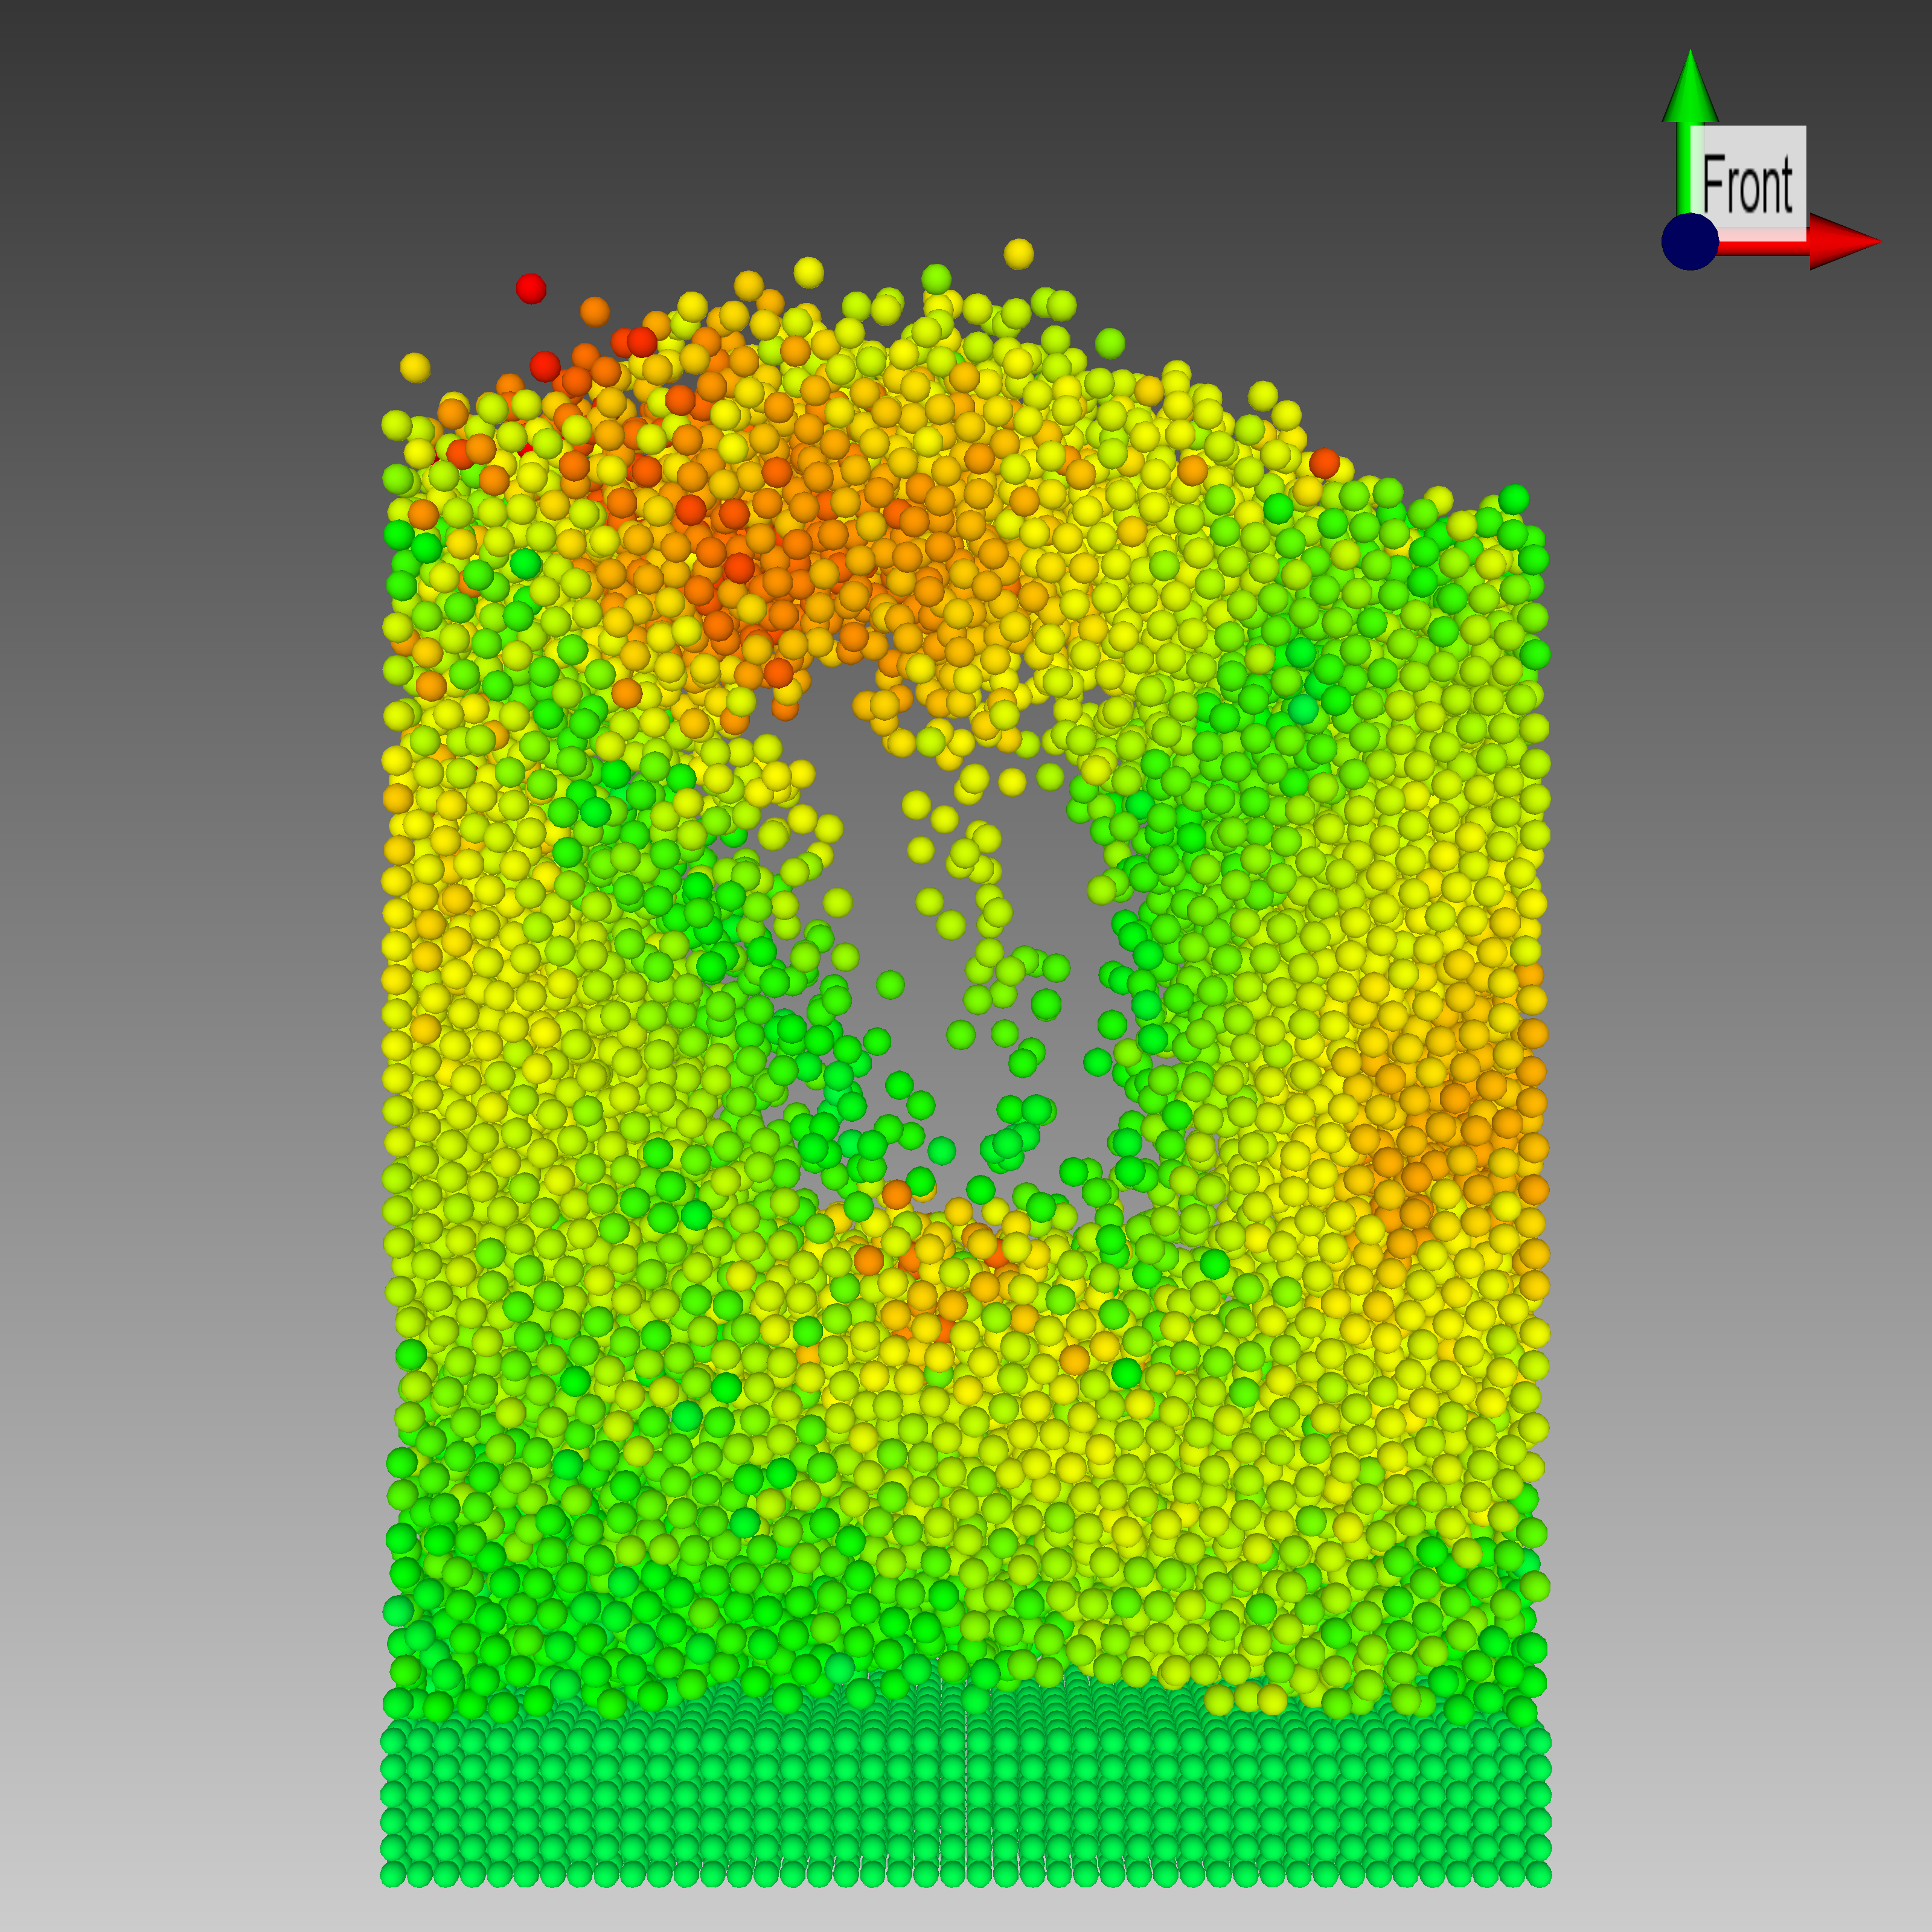
\includegraphics[width=0.2\textwidth]{./figs/particles/new/5.png}
	}
	\hfill
	\subfloat{%
		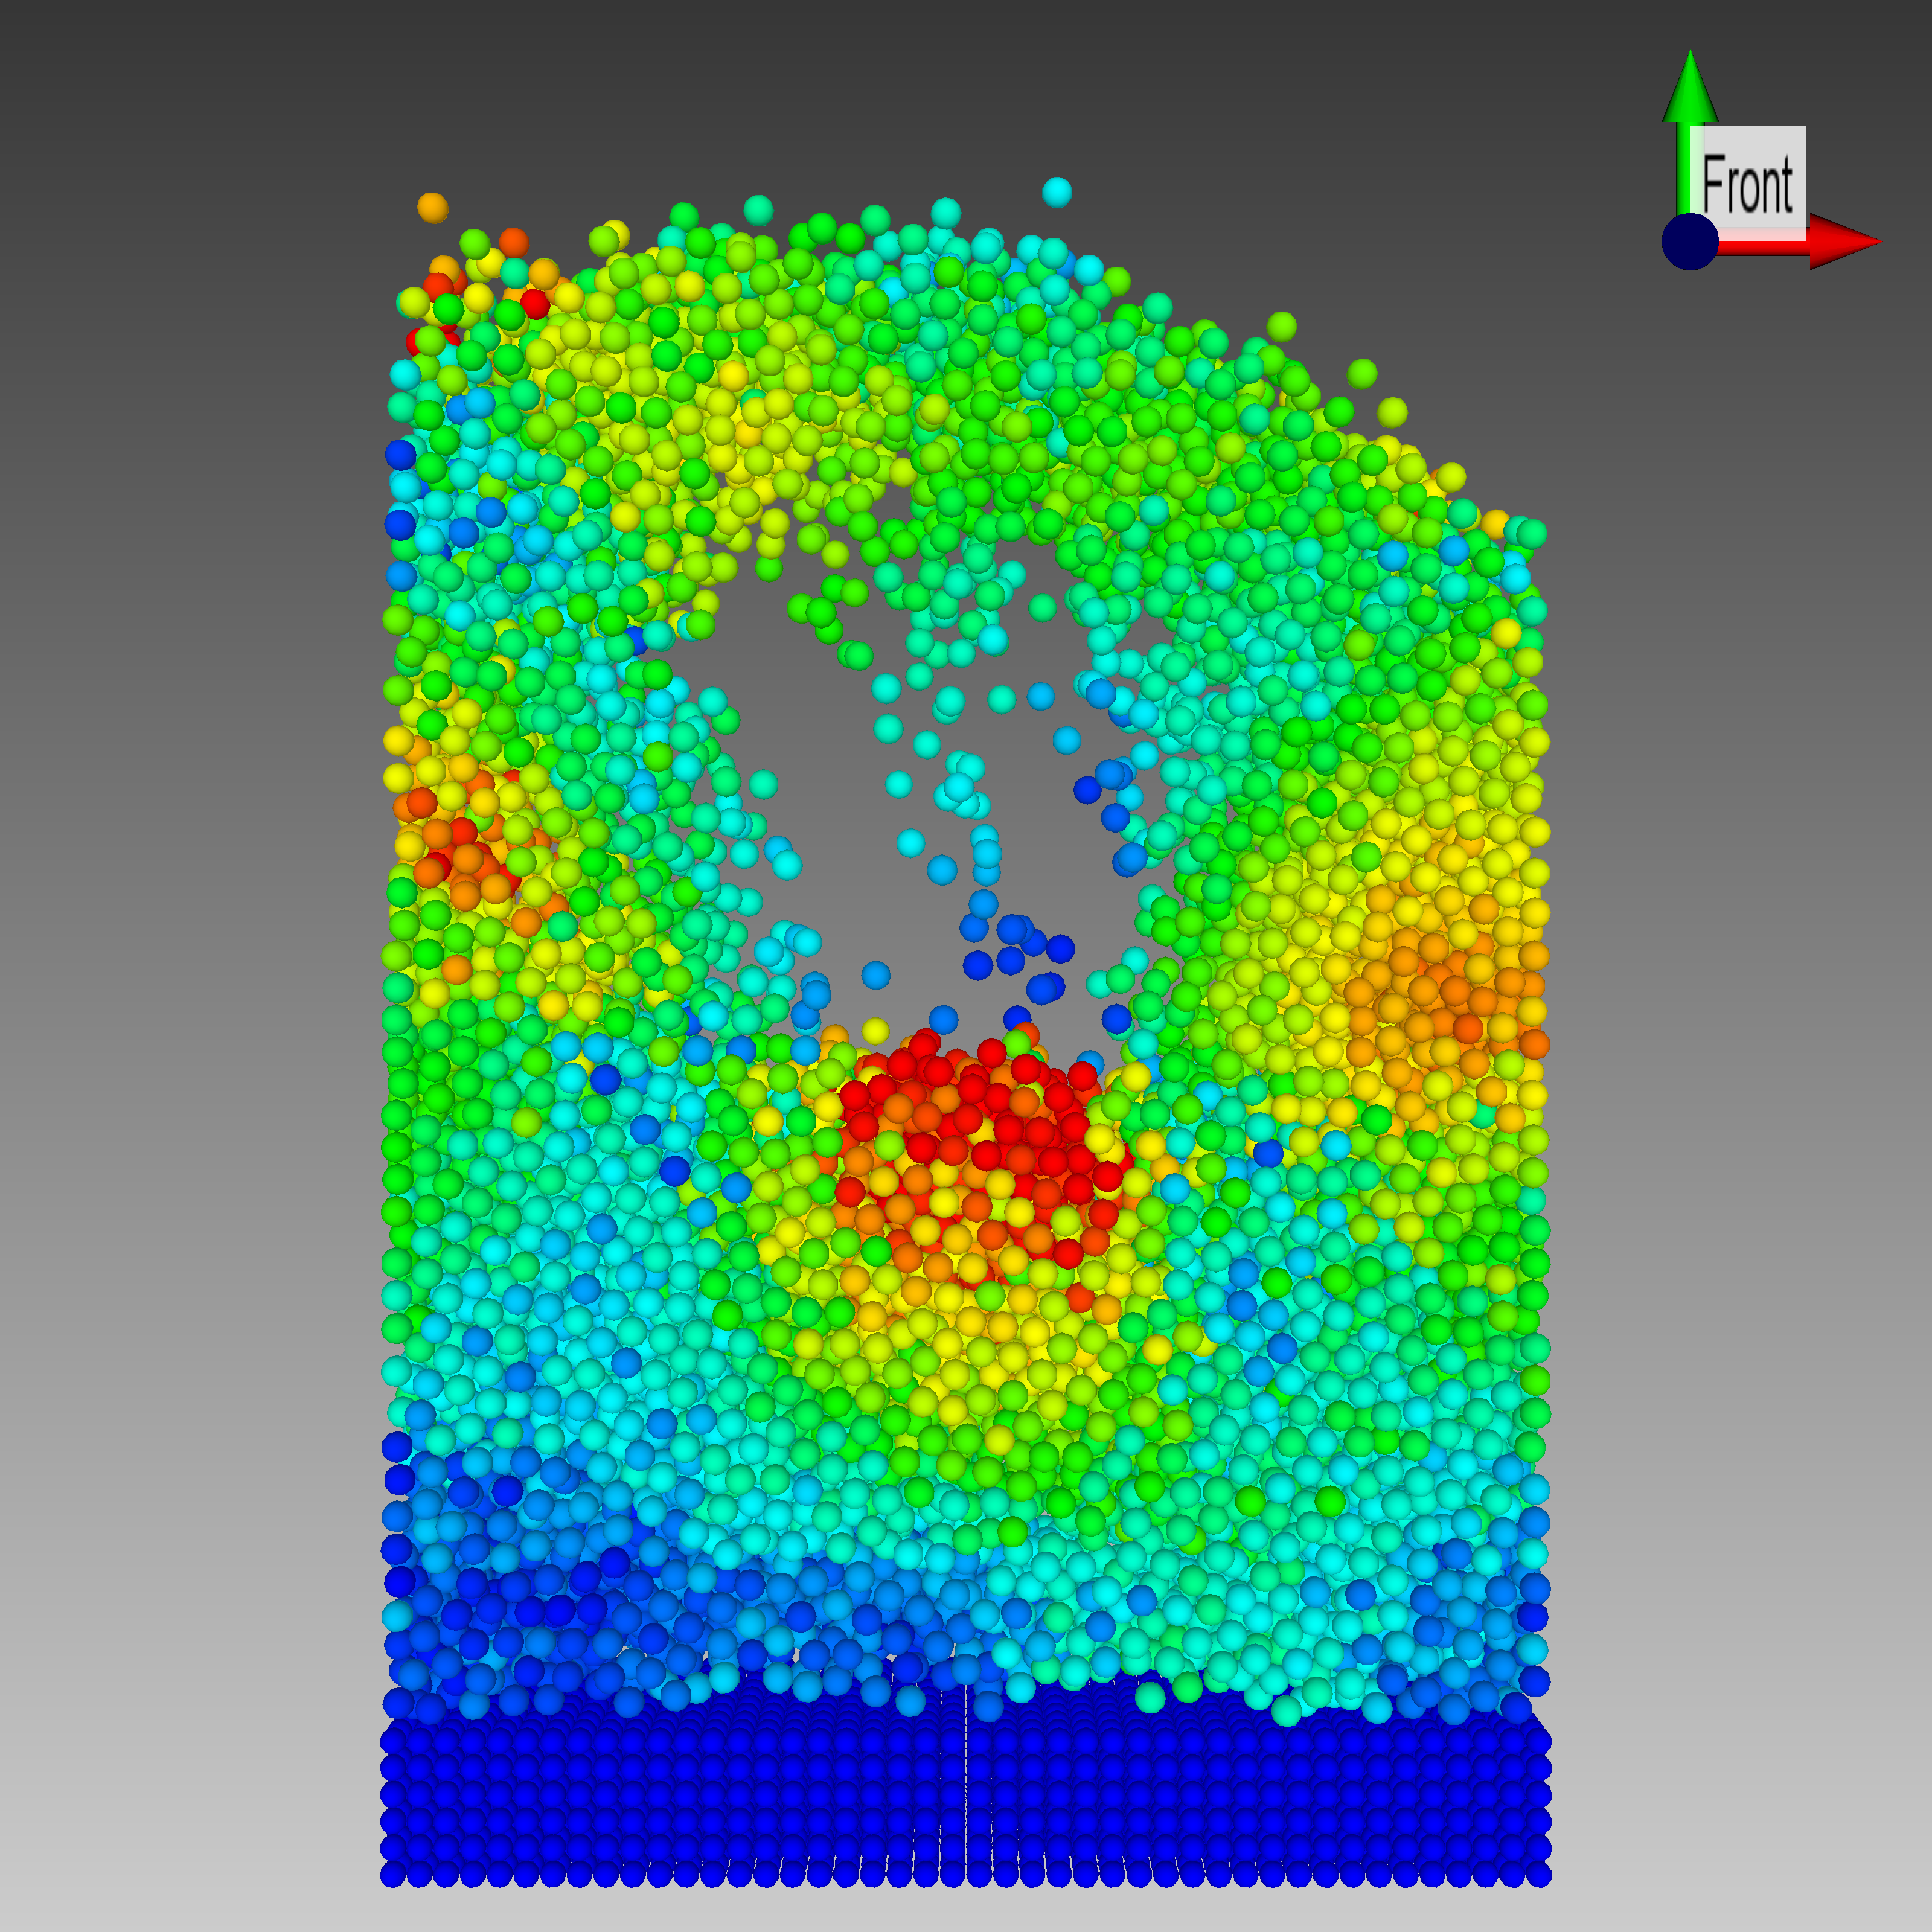
\includegraphics[width=0.2\textwidth]{./figs/particles/new/6.png}
	}
	\hfill
	\subfloat{%
		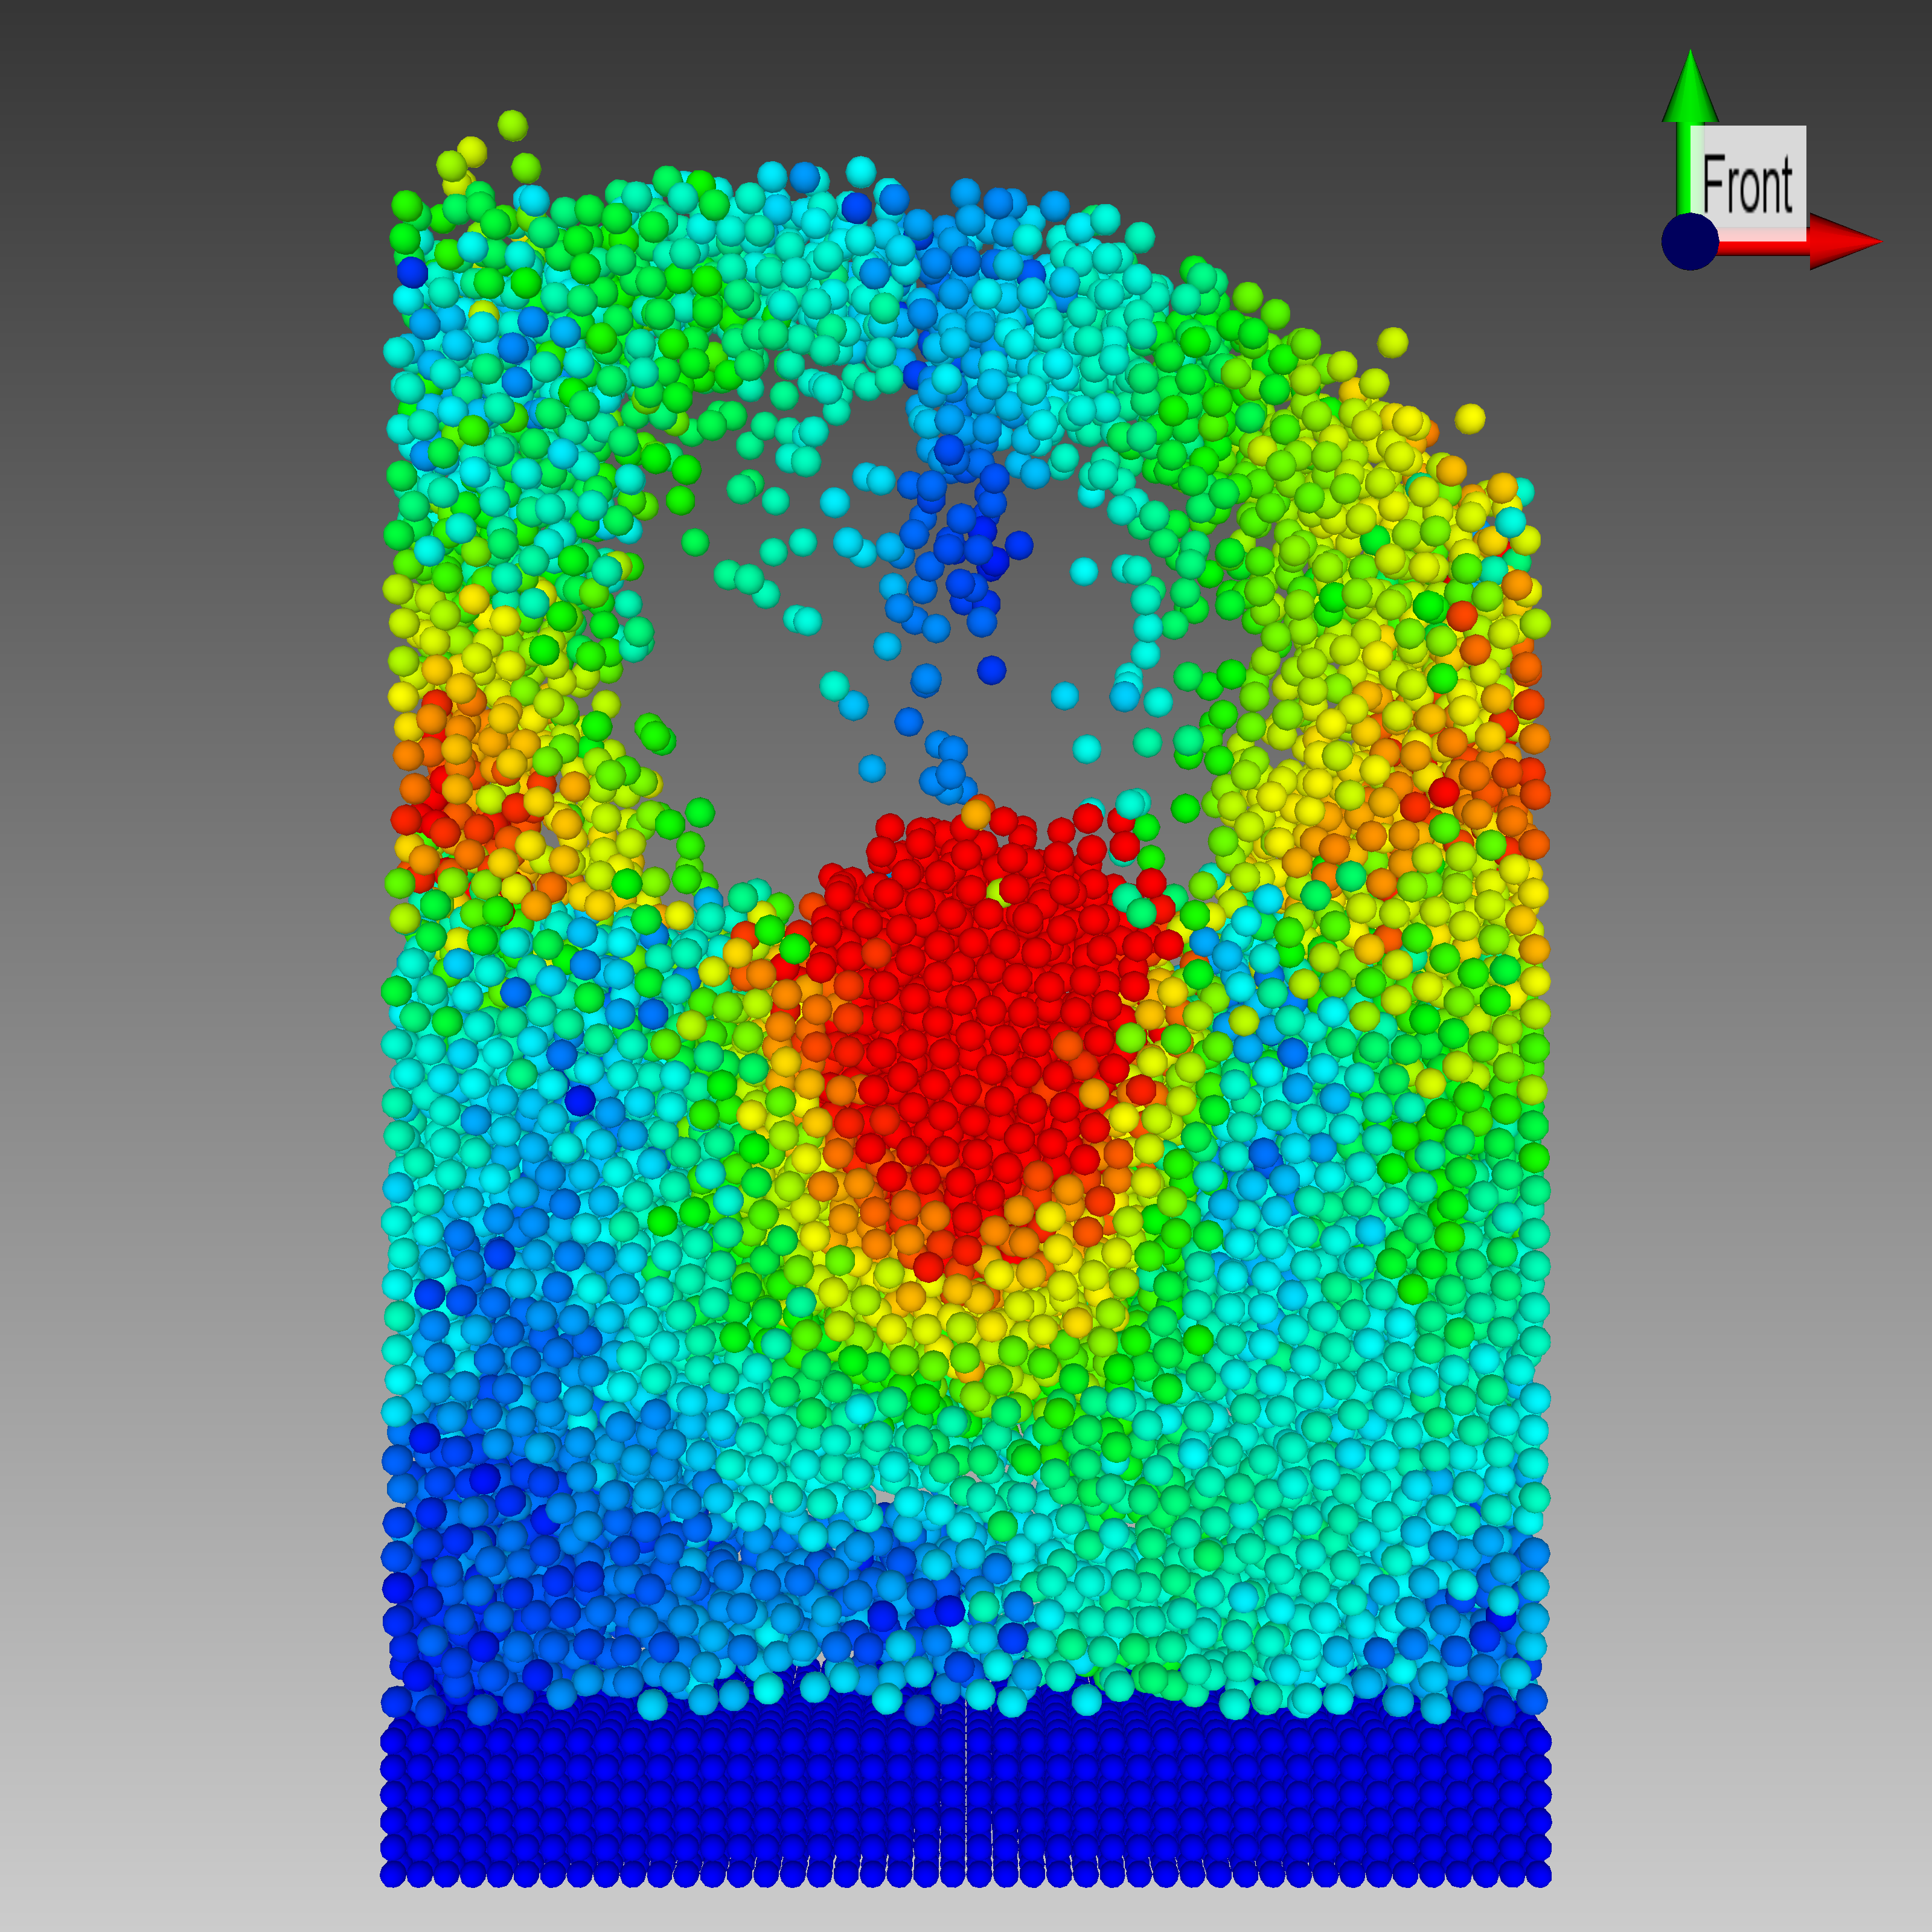
\includegraphics[width=0.2\textwidth]{./figs/particles/new/7.png}
	}
	\hfill
	\subfloat{%
		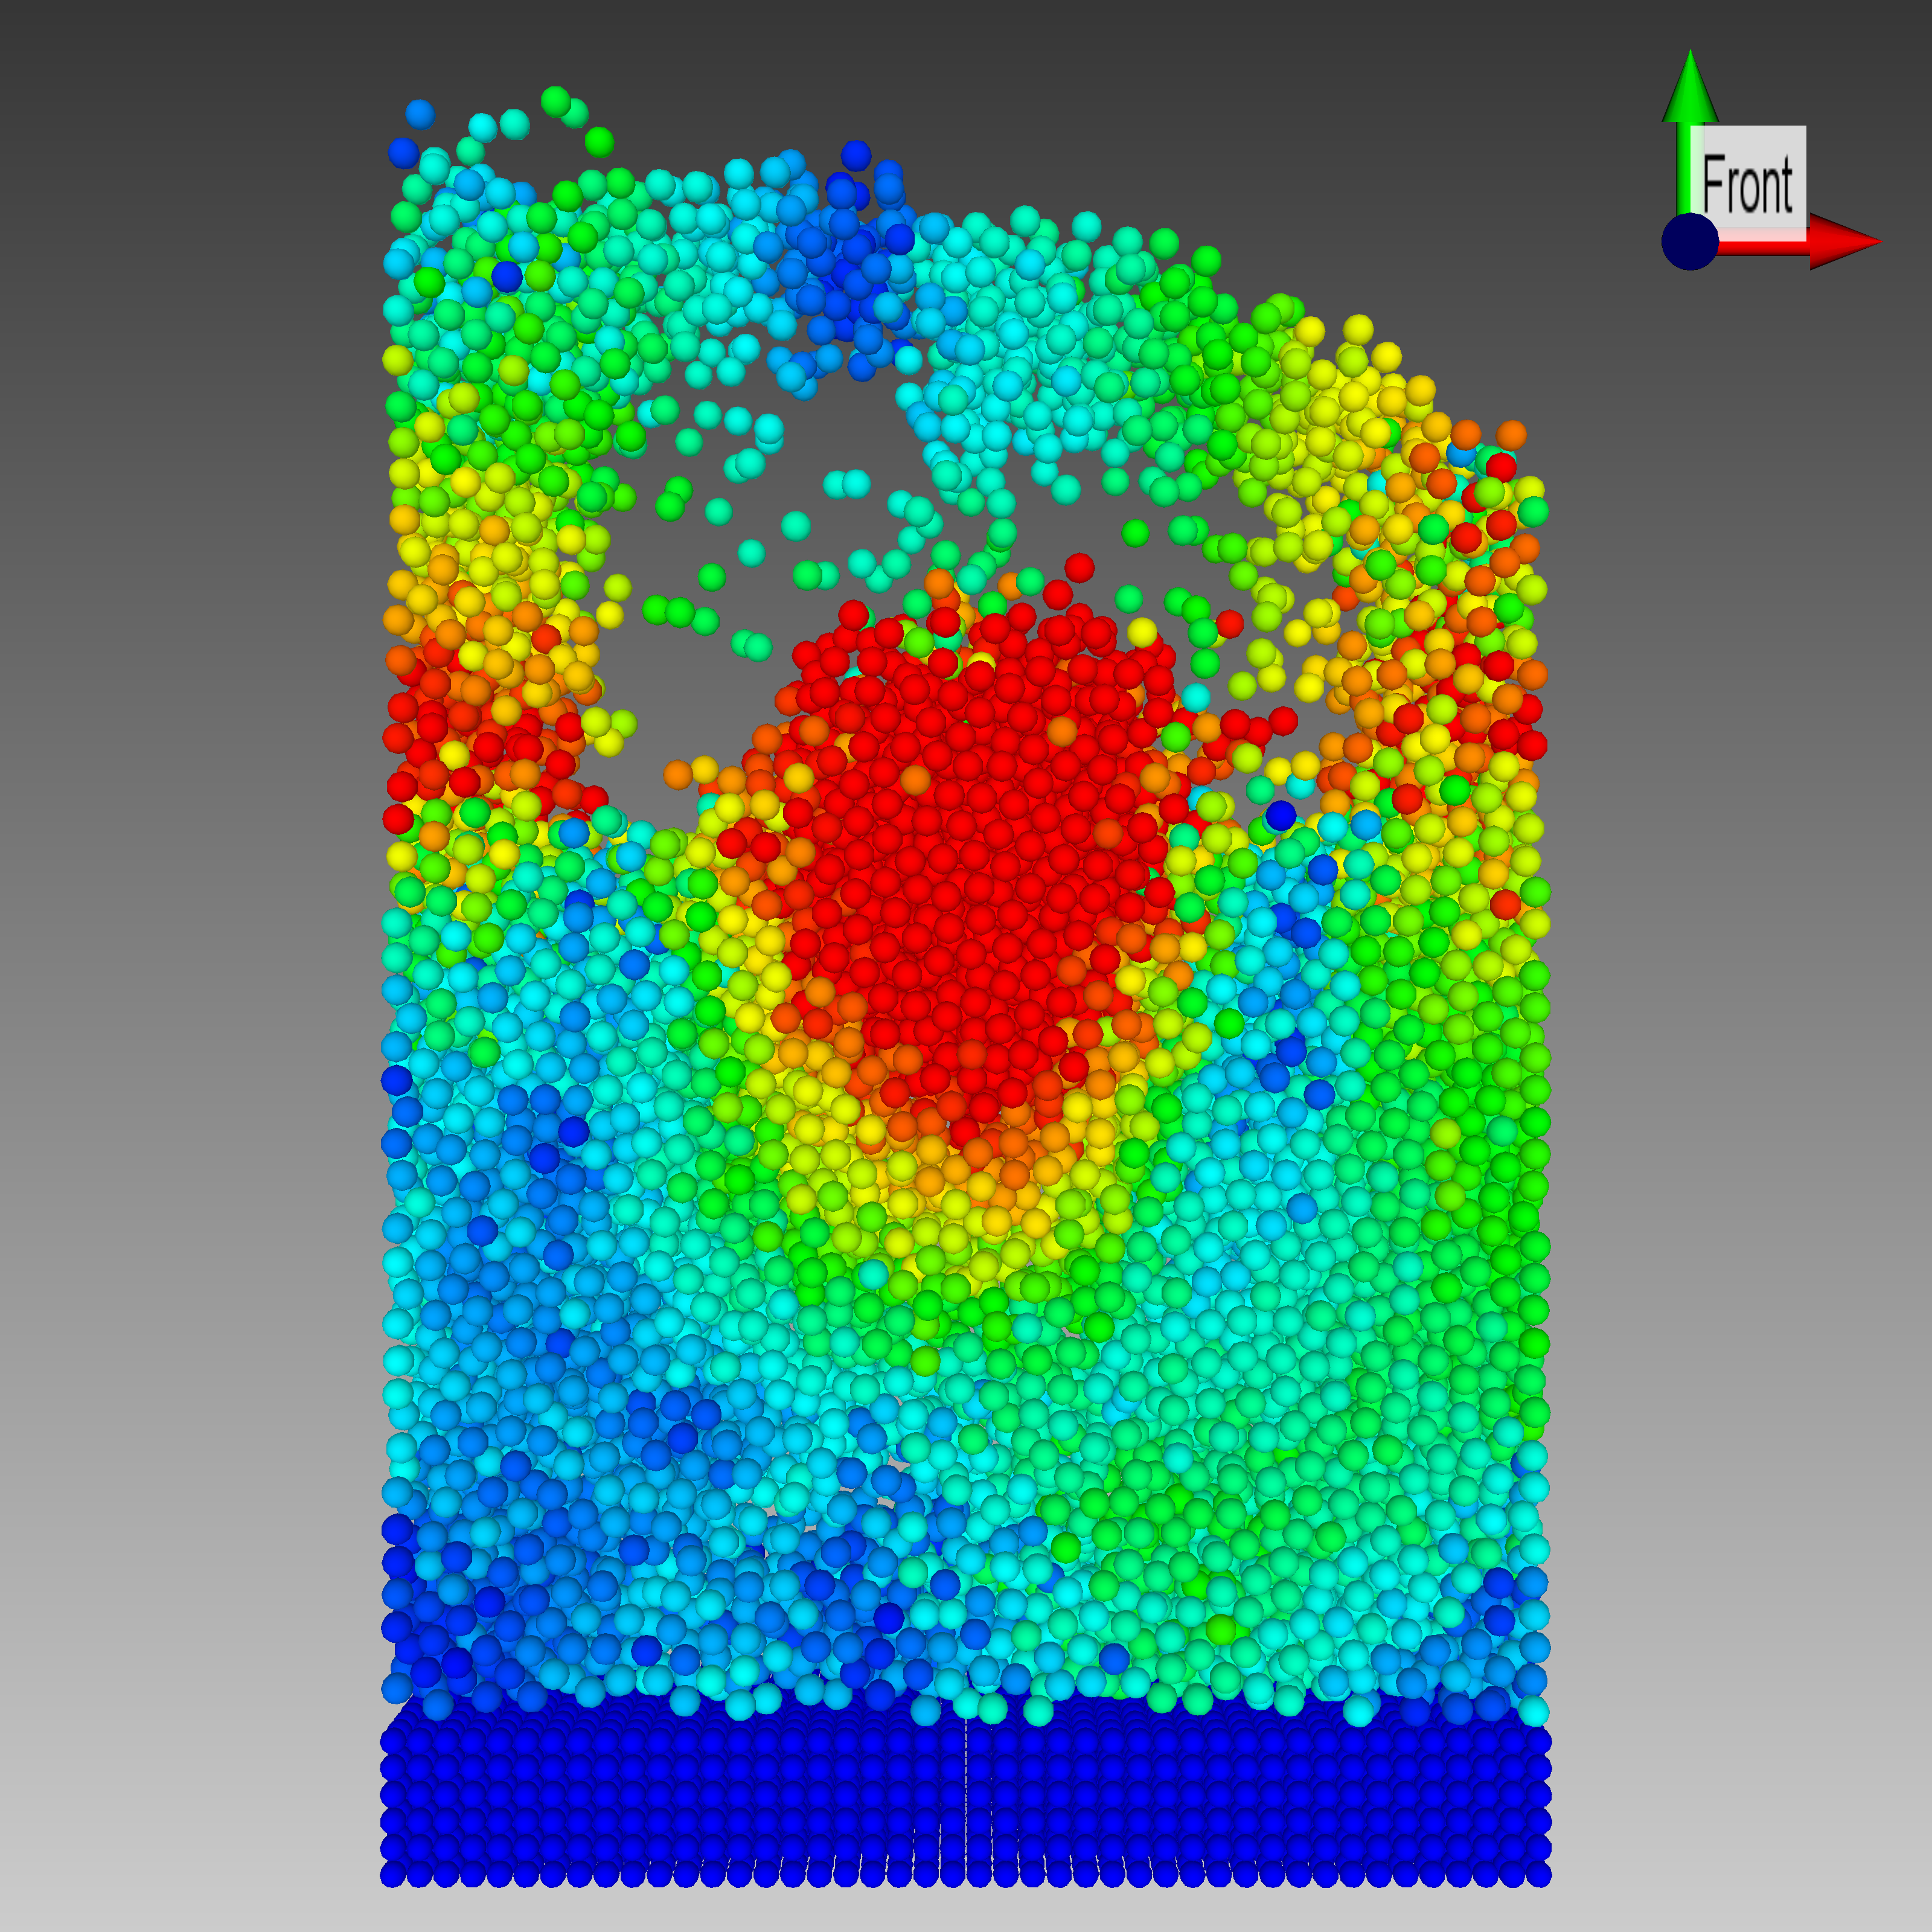
\includegraphics[width=0.2\textwidth]{./figs/particles/new/8.png}
	}
	\hfill
	\subfloat{%
		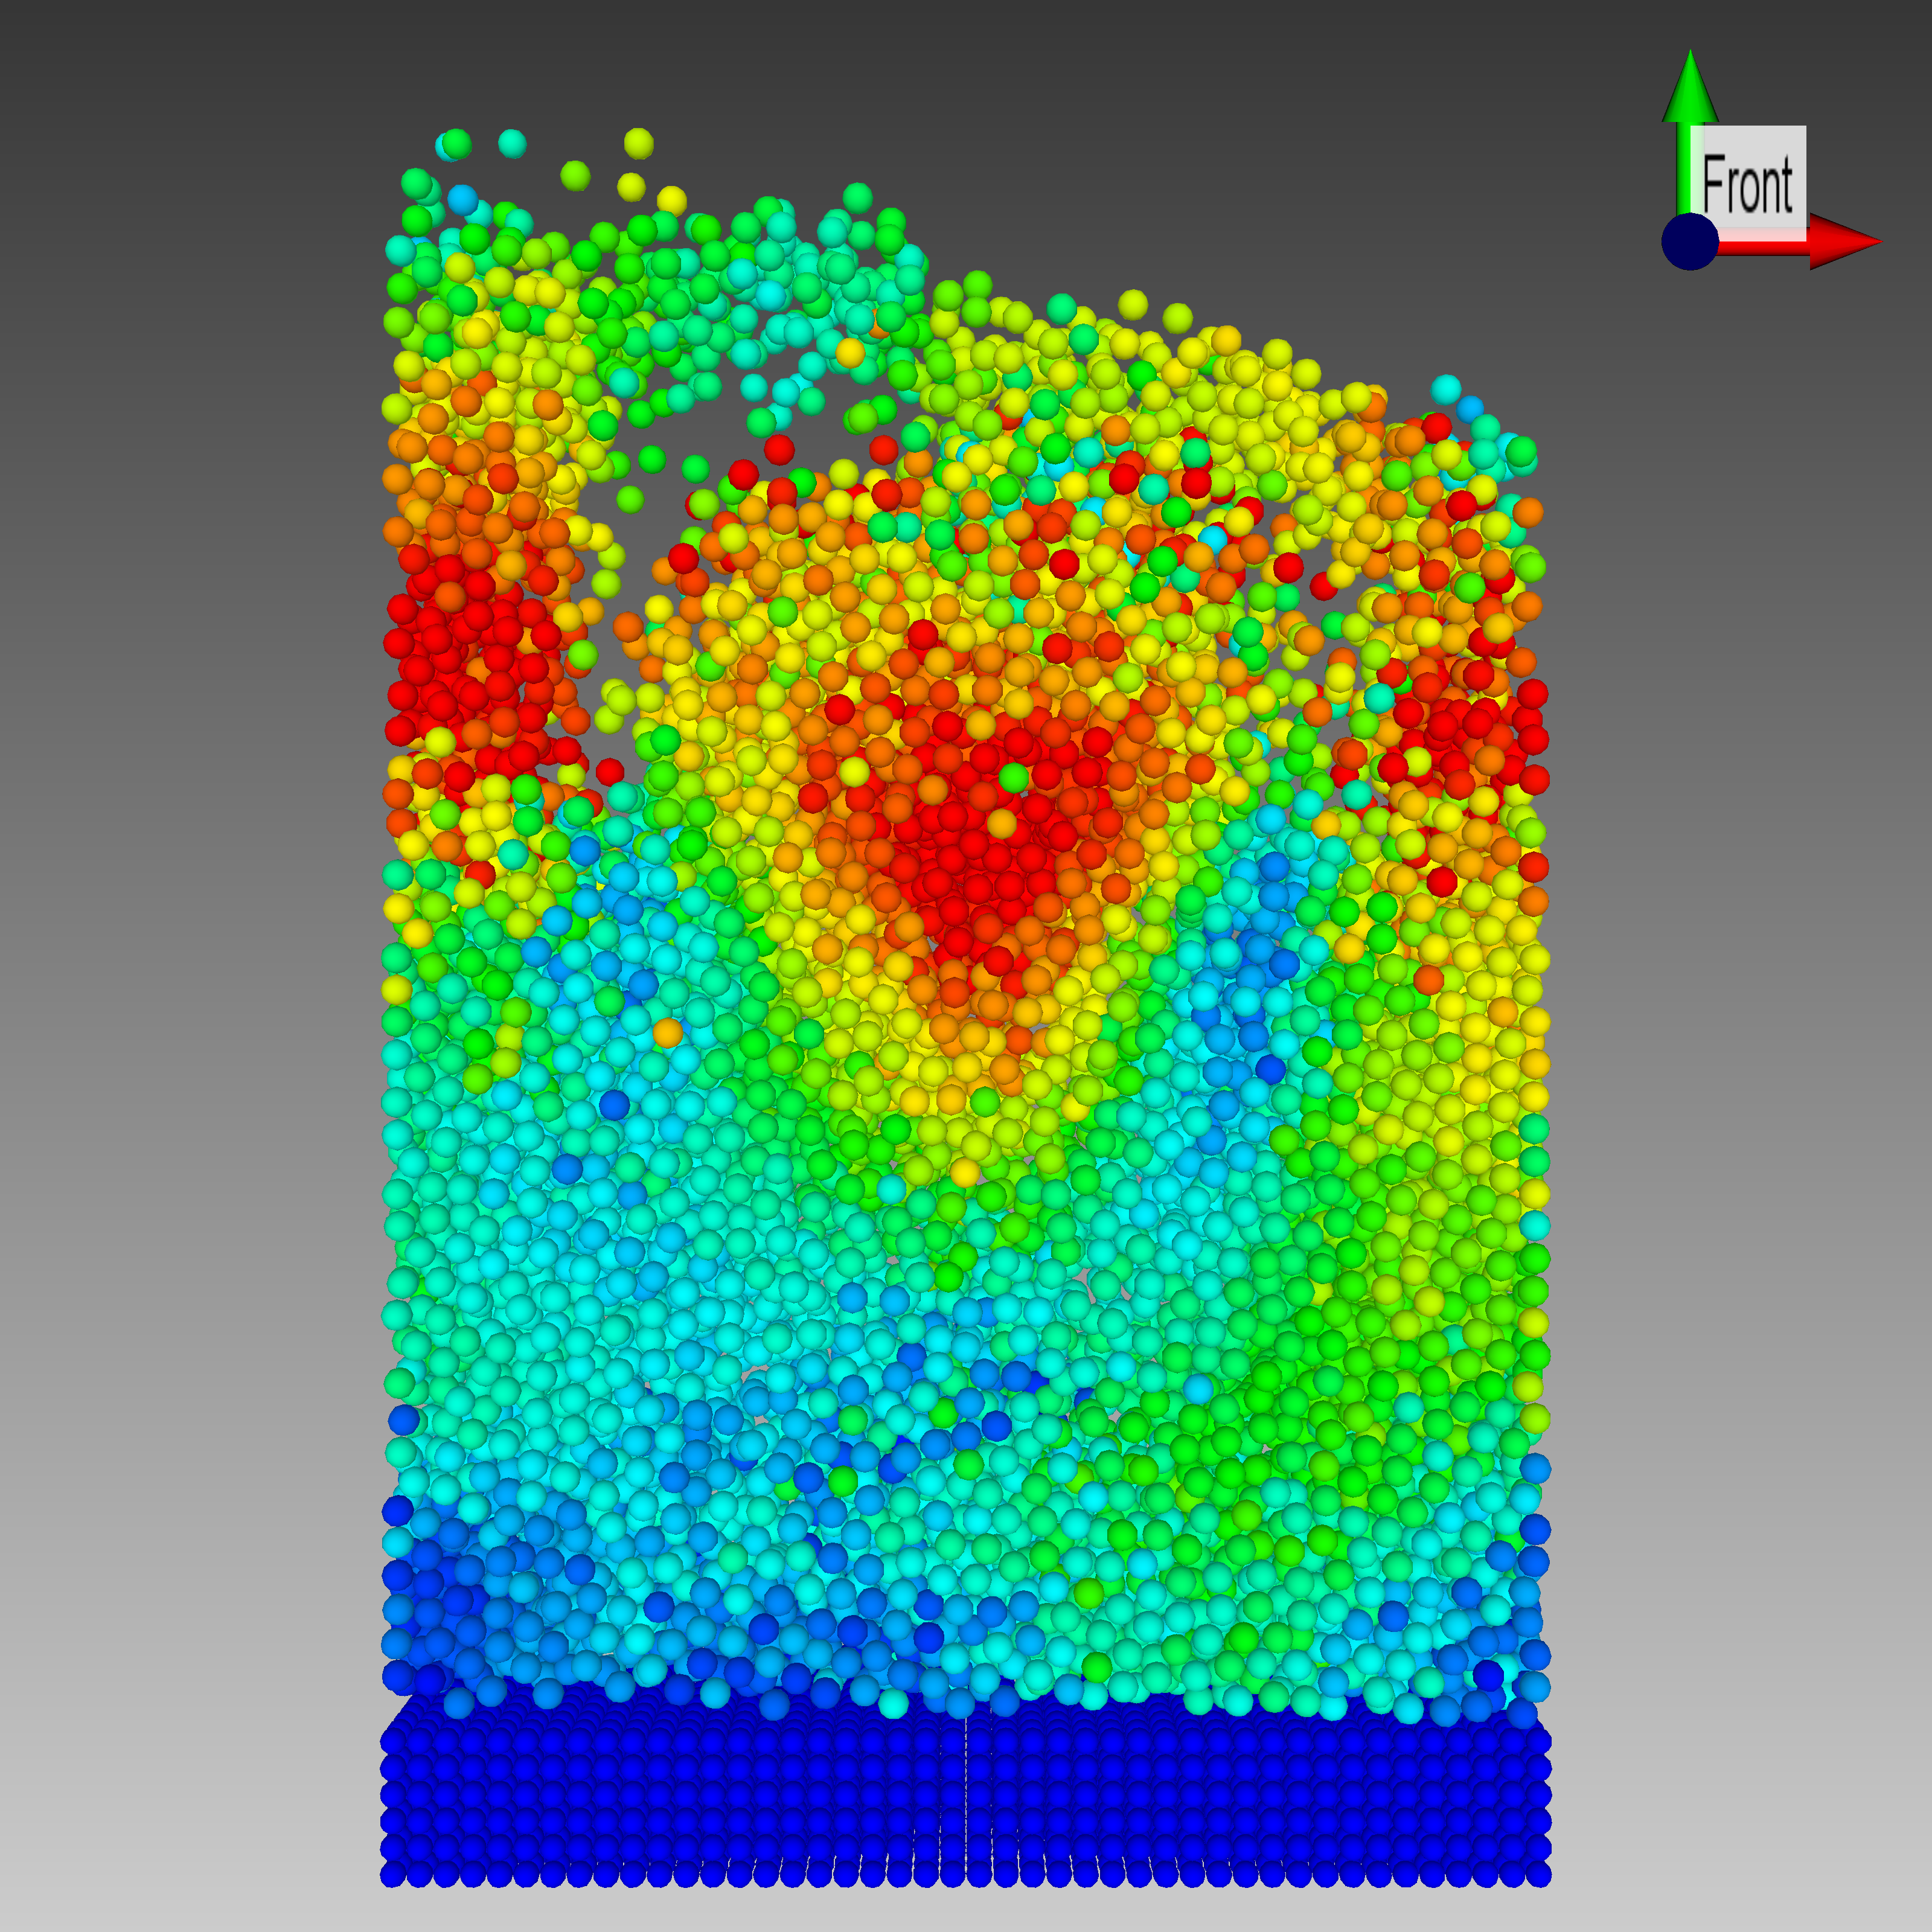
\includegraphics[width=0.2\textwidth]{./figs/particles/new/9.png}
	}
	\hfill
	\subfloat{%
		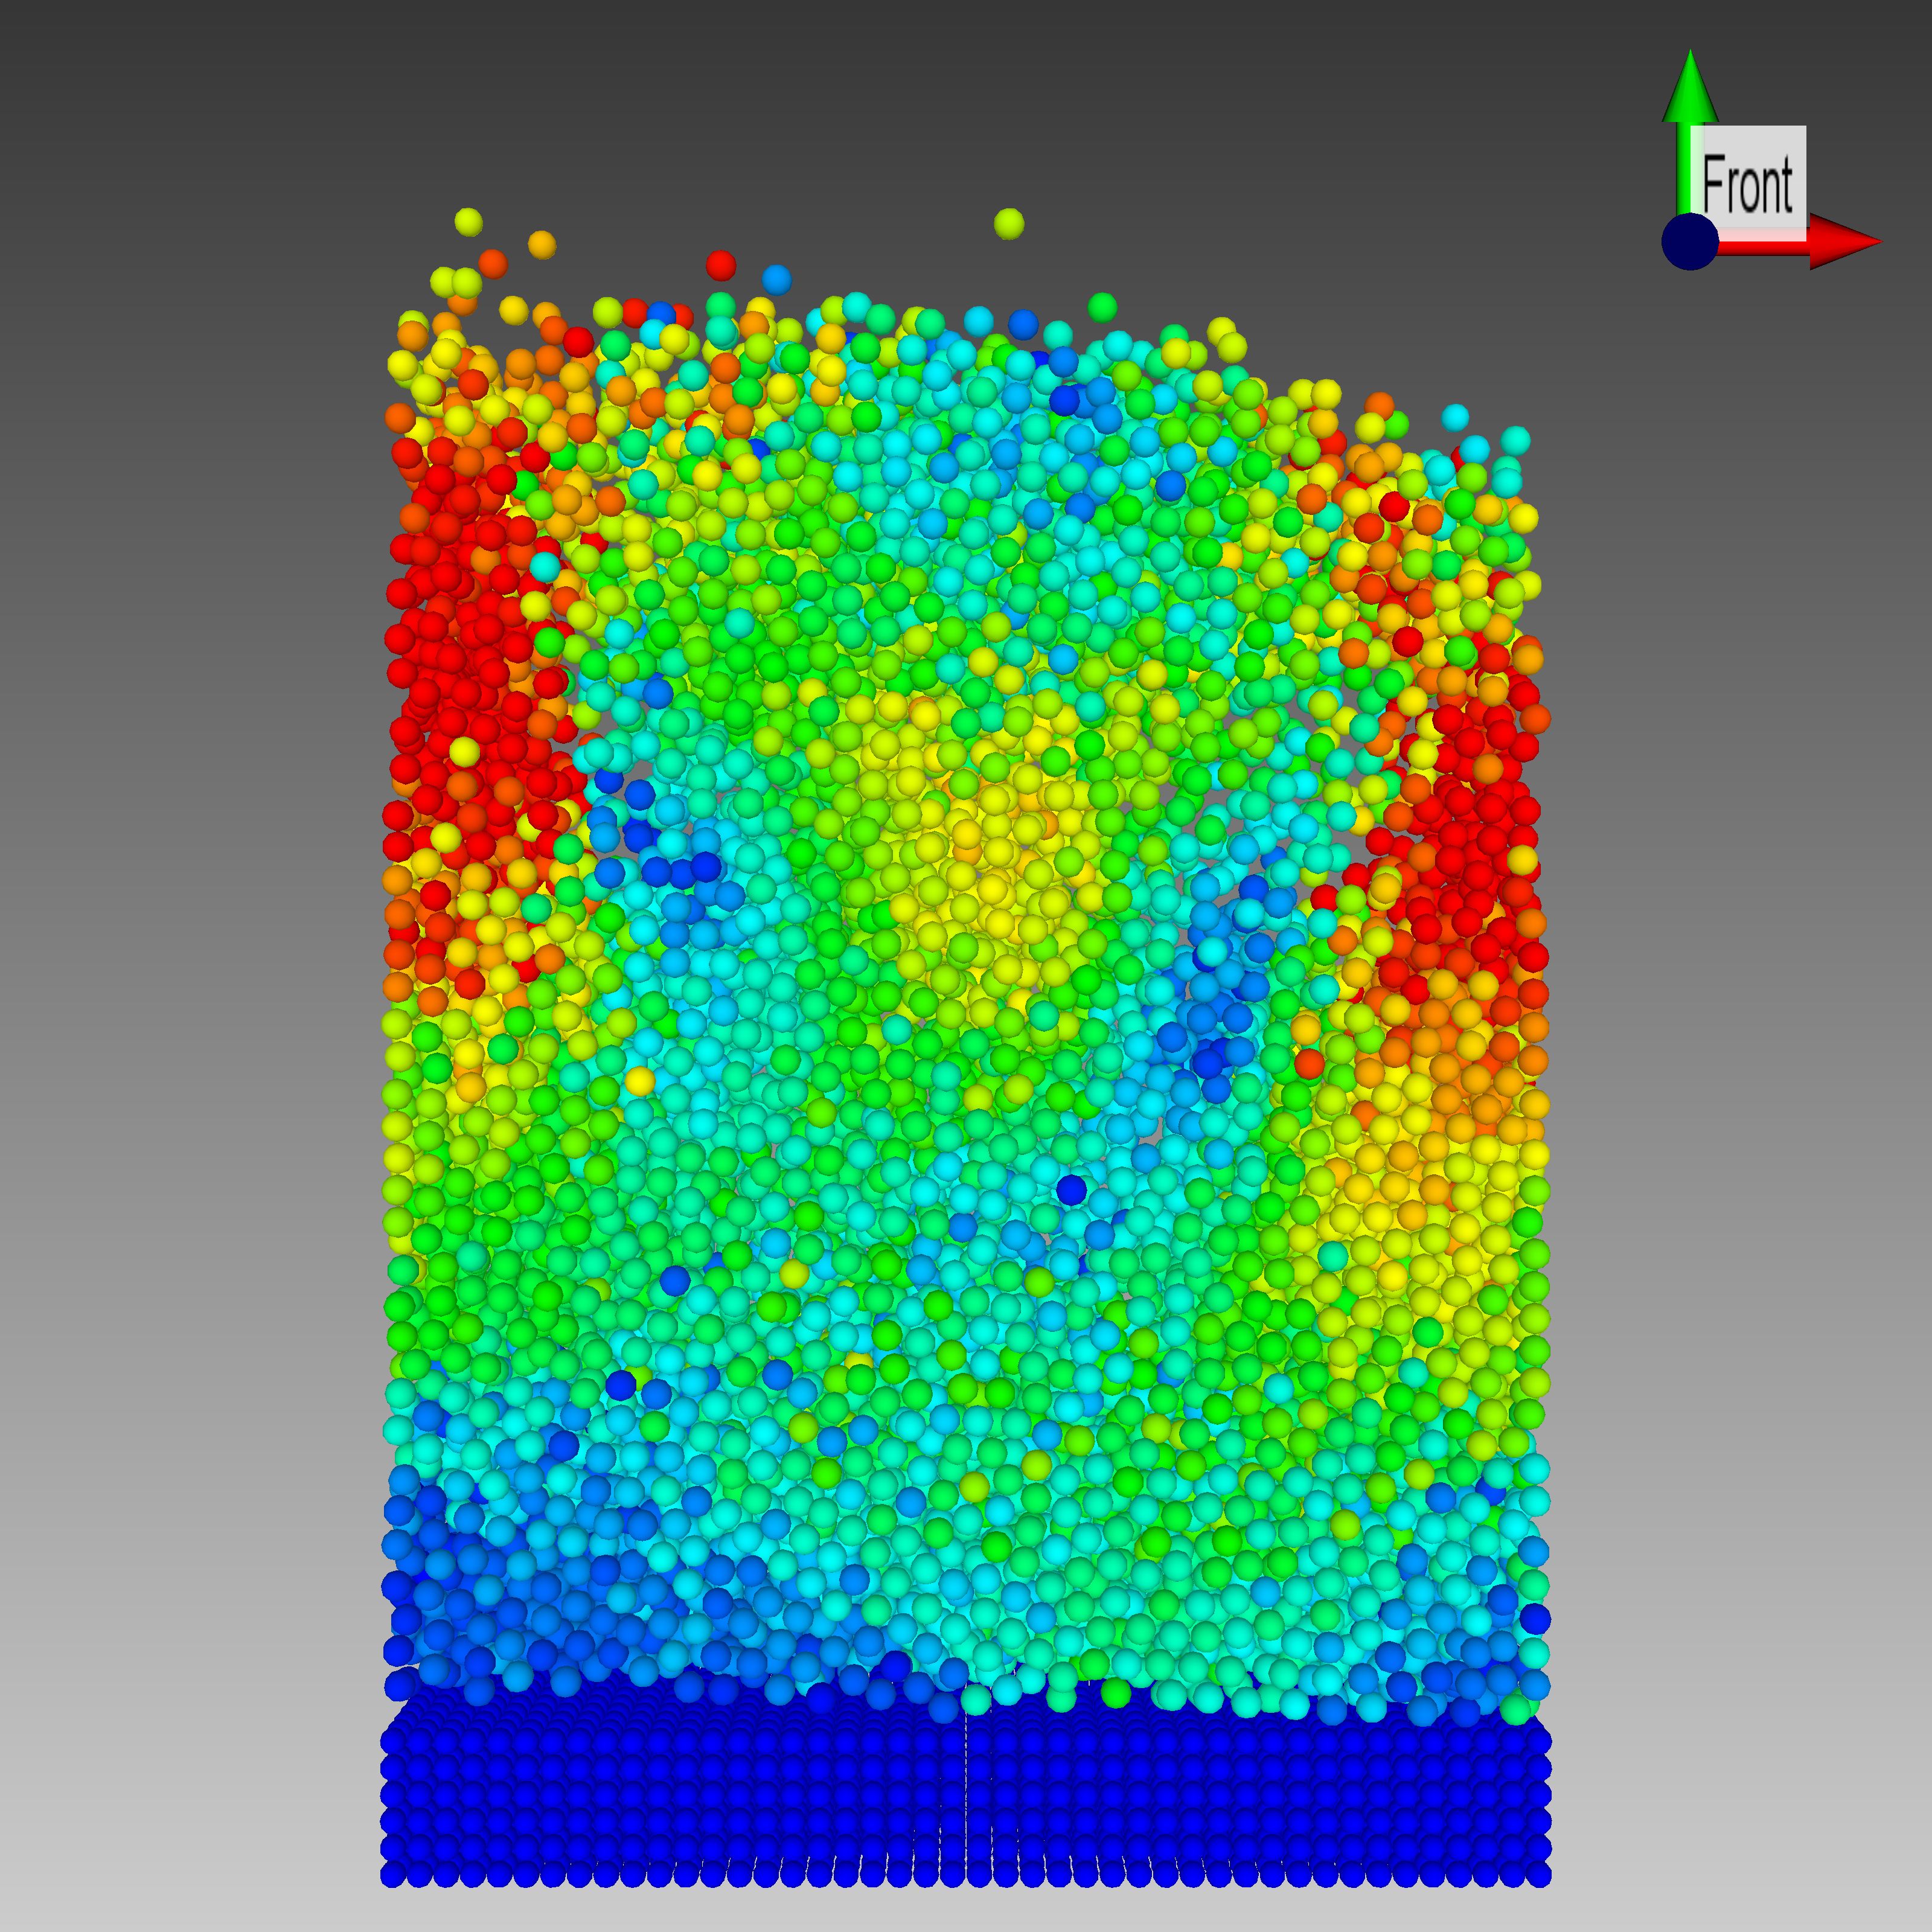
\includegraphics[width=0.2\textwidth]{./figs/particles/new/10.png}
	}
	\hfill
	\subfloat{%
		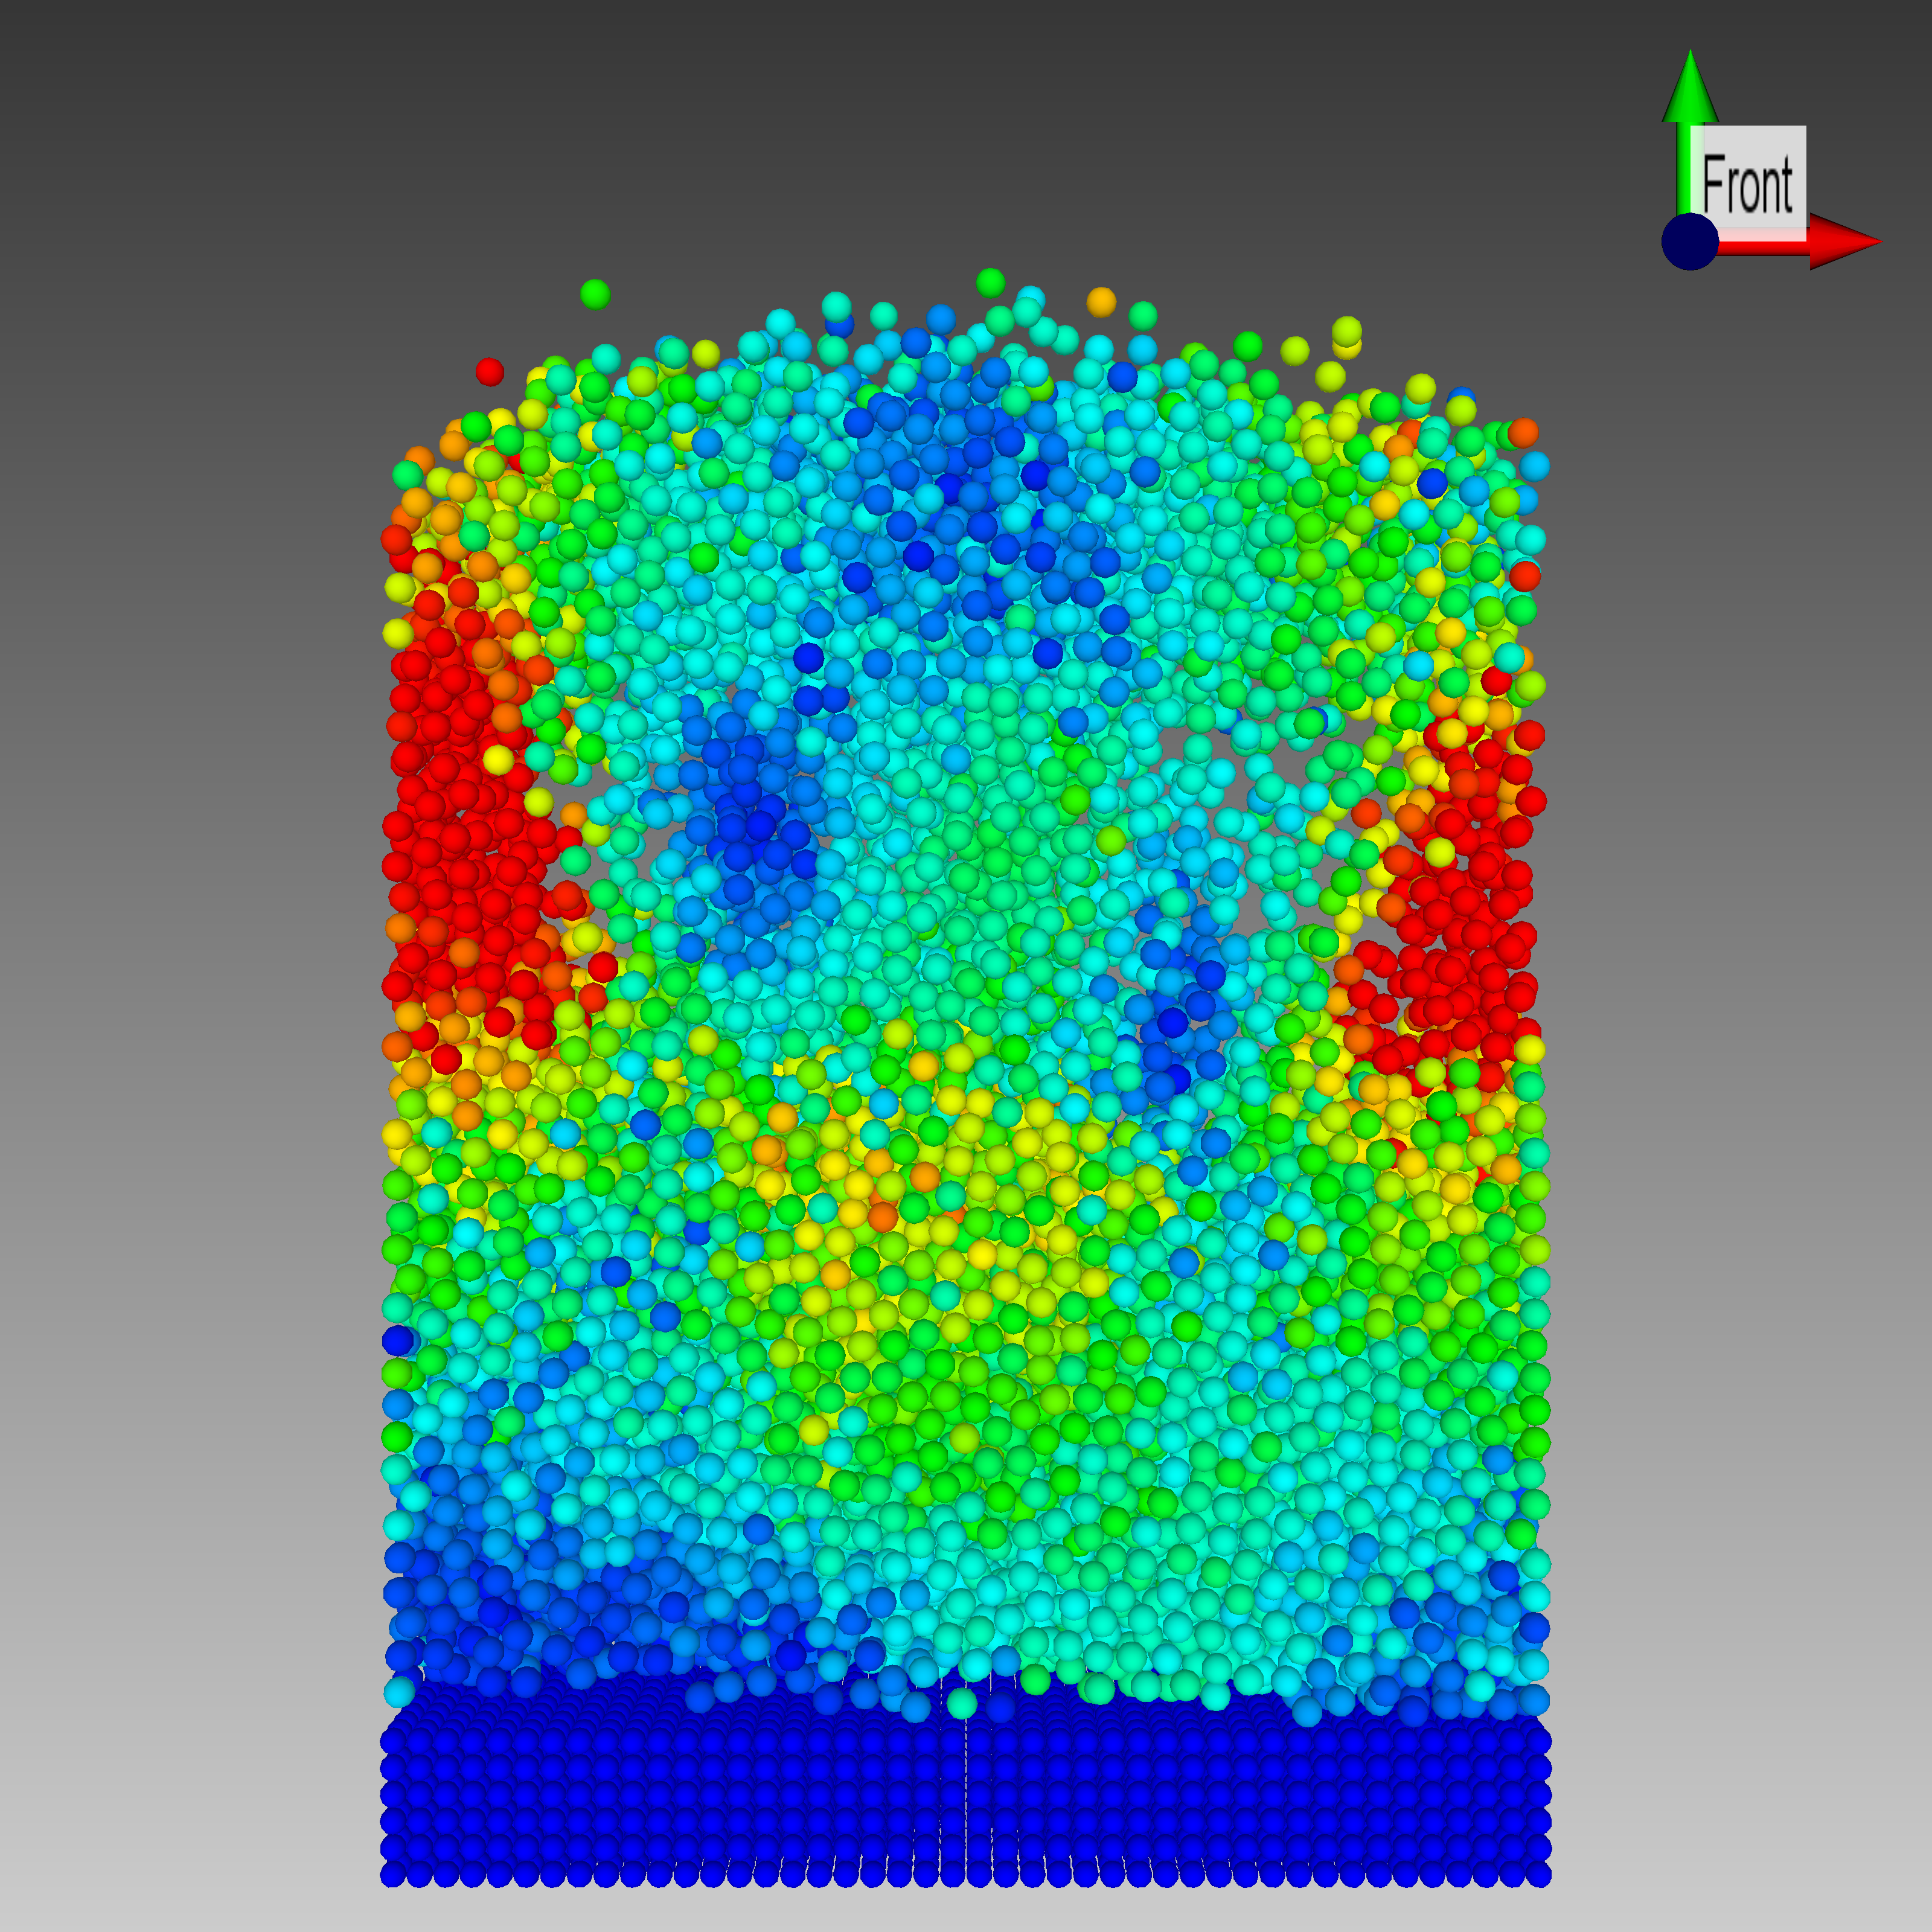
\includegraphics[width=0.2\textwidth]{./figs/particles/new/11.png}
	}
	\hfill
	\subfloat{%
		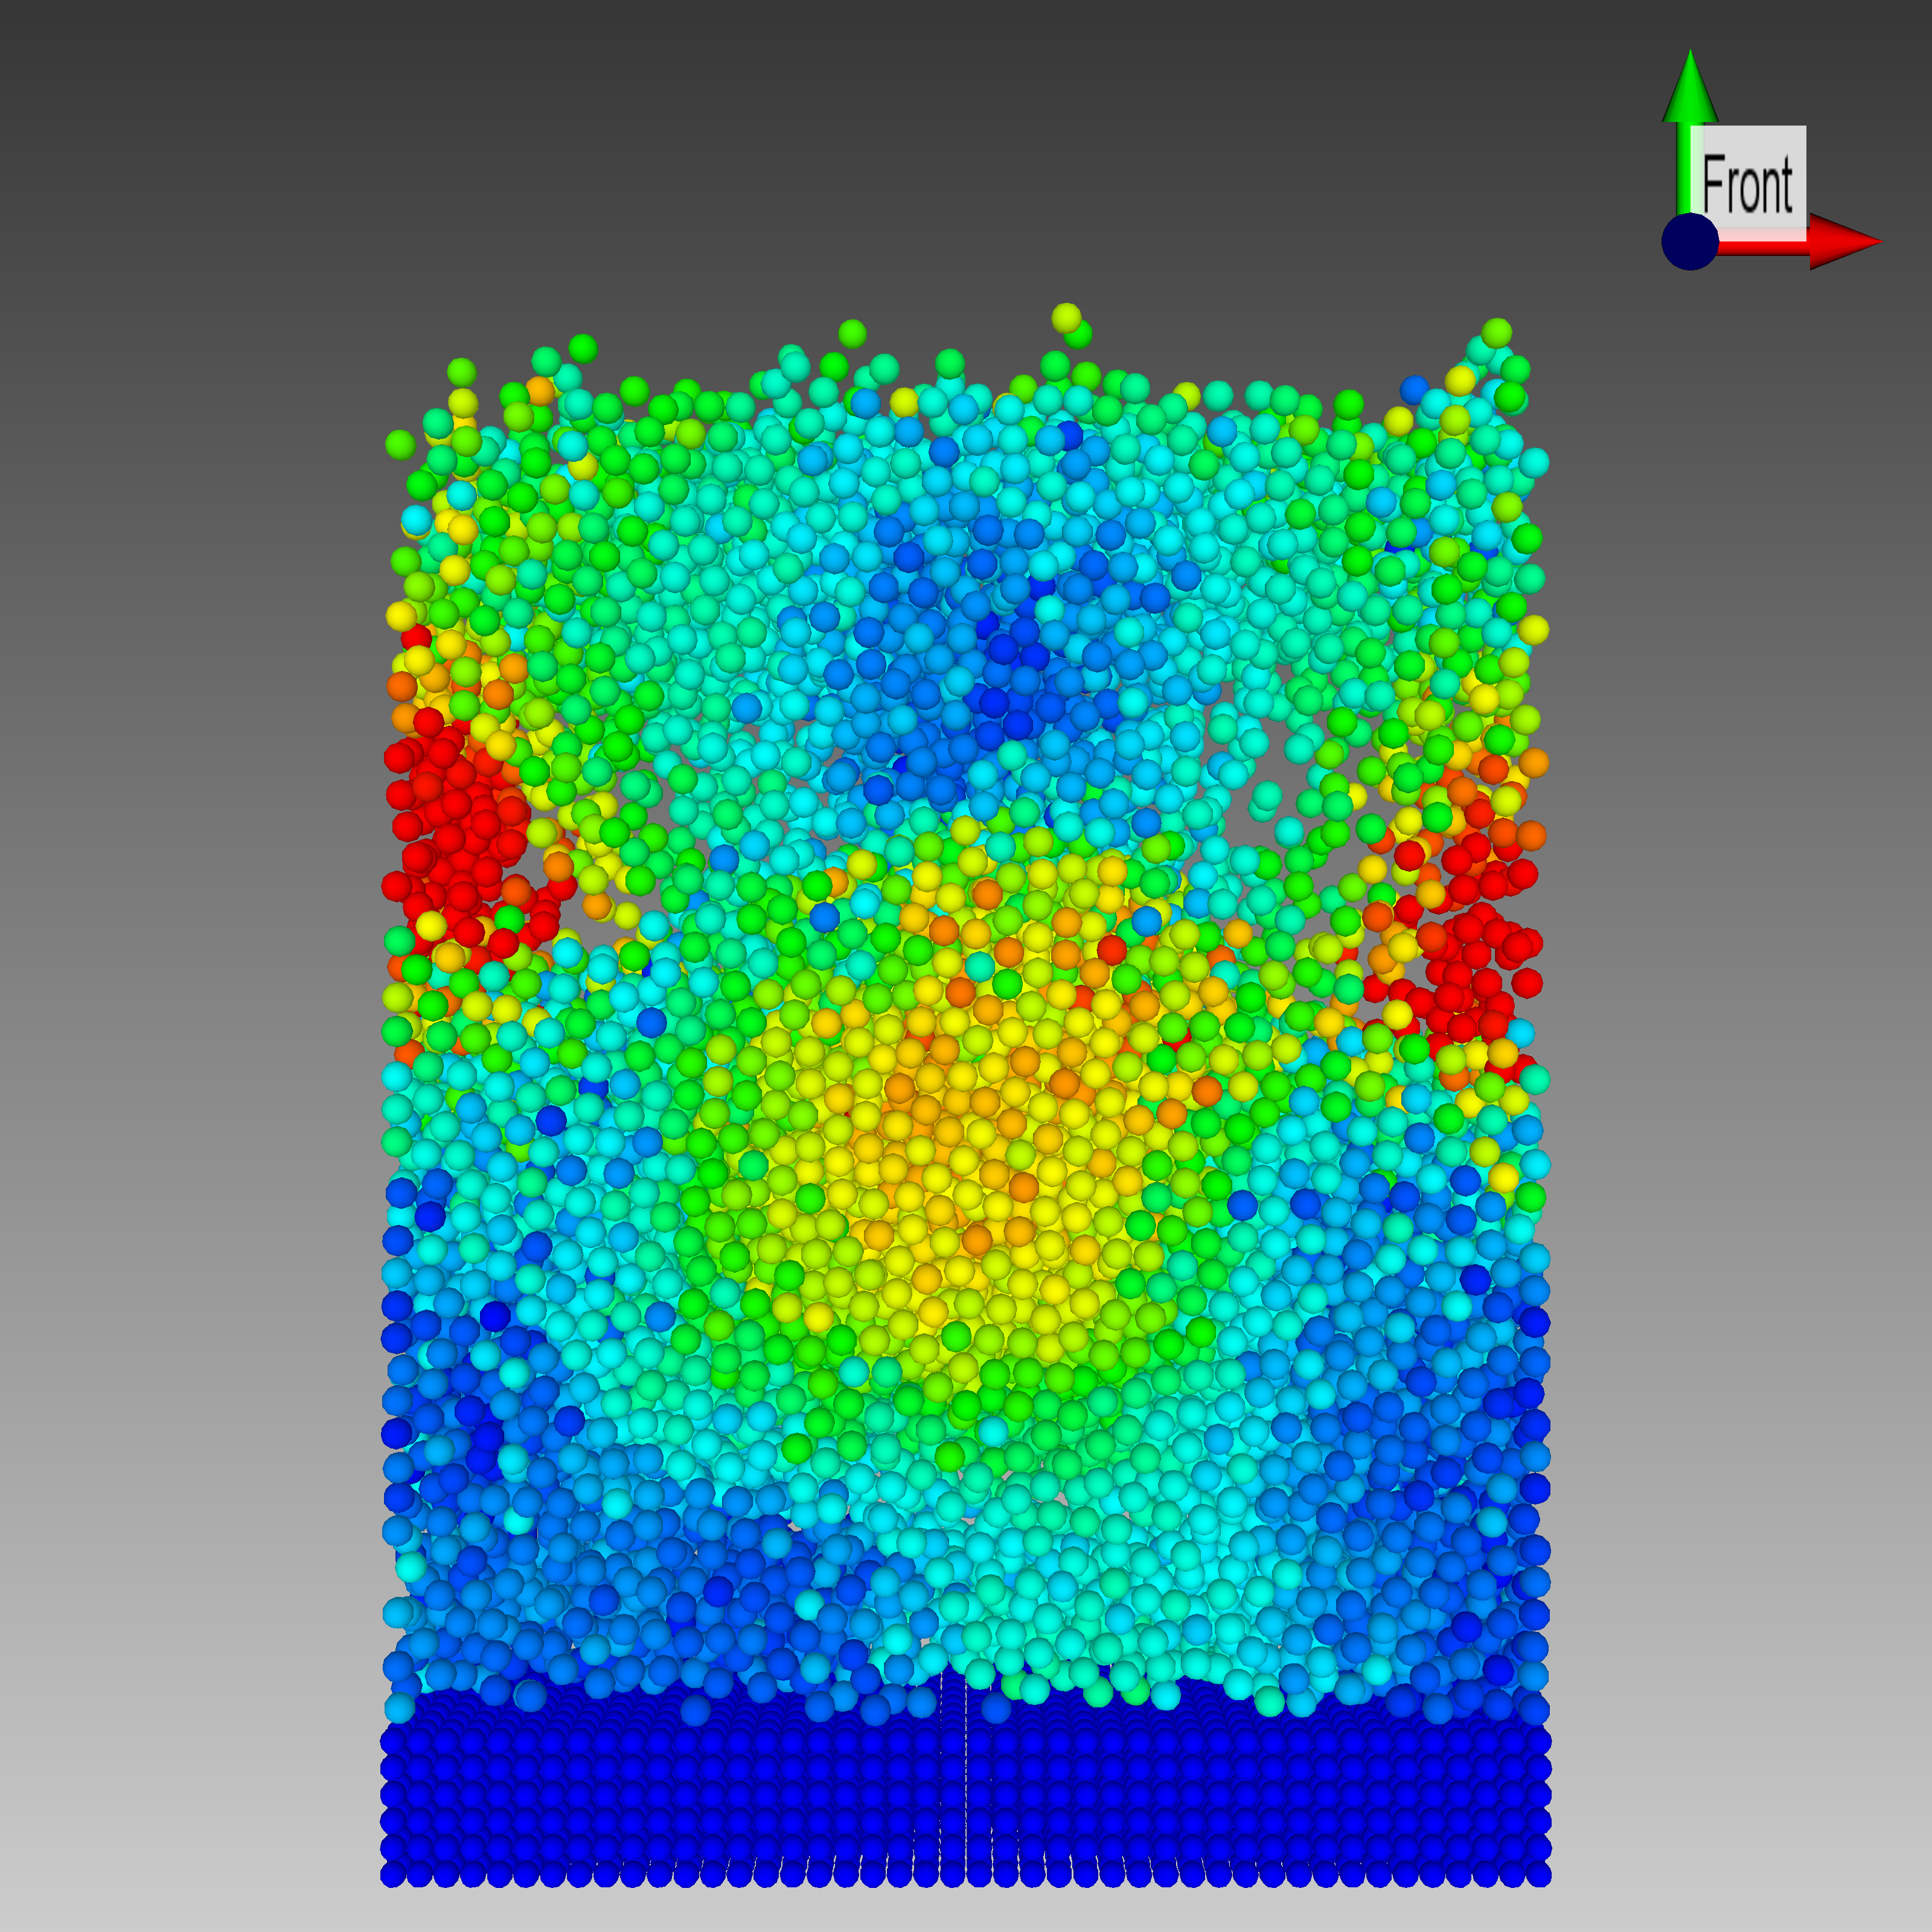
\includegraphics[width=0.2\textwidth]{./figs/particles/new/12.png}
	}
	\hfill
	\caption[Virtual Reality]{\textbf{Particle Visualization} in VELaSSCo.}
	\label{fig:particles}
\end{figure}

\textbf{VELaSSCo project}. "Visualization for Extremely Large Scale Scientific Computing" known as VELaSSCo is an EC funded project which deals with end-user visualization of Big Data. The idea behind this project is to store the datasets on a distributed database like HBase (Hadoop) or EDM. The user can query a specific part of data in the database or a specific operation on the data in the database,e.g.~Figure XX show the query for boundary mesh of telescope dataset which is processed on the fly on HPC and then the data is being transfered directly to the user computer or being stored in the database.

In this project, I mainly focused on implementing two direct result queries used for querying results on a specific vertex indices, and querying mesh draw data for models in the database. Mesh drawing data query result needed to be returned in a GPU friendly format, so the received data on the client side can be copied directly into an OpenGL buffer directly. I implemented these two queries using Thrift C++ API. On the client side, I implemented a plug-in to support VELaSSCo Plugin for indoor application called Rapid Prototyping Environment (RPE). This plugin is able to:

\begin{itemize}
	\item query for available models, their analysis, results, meshes, and static meshes.
	\item Query for computing boundary mesh of a specific dataset.
	\item Query for Finite Element Meshes (FEM) / Discrete Element Meshes (DEM) and render them.
	\item Query for results on a specific node (or evaluation in all time steps).
	\item Query for different timesteps for DEM cases and create an animation.
\end{itemize}

\begin{figure}[!ht]
	\centering
	\includegraphics[width=0.90\textwidth]{./figs/pipecube.png}
	\caption[Pipecube]{\textbf{Pipecube} made of more than 15.6 million pipes, ray-traced on Full HD on 17 fps using Intel Embree on a Intel Core i7-4960X.}
	\label{fig:pipecube}
\end{figure}

\begin{figure}[!ht]
	\subfloat{%
		\includegraphics[width=0.3\textwidth]{./figs/embree1.png}
	}
	\hfill
	\subfloat{%
		\includegraphics[width=0.3\textwidth]{./figs/embree2.png}
	}
	\hfill
	\subfloat{%
		\includegraphics[width=0.3\textwidth]{./figs/embree3.png}
	}
	\hfill
	\caption[Factory ray-tracing]{\textbf{Factory ray-tracing with Embree}.}
	\label{fig:embreeFactory}
\end{figure}

\begin{figure}[!ht]
	\subfloat{%
		\includegraphics[width=0.3\textwidth]{./figs/optix1.png}
	}
	\hfill
	\subfloat{%
		\includegraphics[width=0.3\textwidth]{./figs/optix2.png}
	}
	\hfill
	\subfloat{%
		\includegraphics[width=0.3\textwidth]{./figs/optix3.png}
	}
	\hfill
	\caption[Factory ray-tracing]{\textbf{Factory ray-tracing with Optix}.}
	\label{fig:embreeFactory}
\end{figure}

\textbf{Ray-tracing higher-order primitives}. This task starts with a simple example which was rendering of a pipecube using pipes which are made of two spheres and one cylinder. The GPU version was implemented by Andreas Dietrich and I implemented the CPU version using Intel Embree. The CPU version was able to handle very big pipecubes (Figure \ref{fig:pipecube}). This was an starting idea for implementing a version which uses the AVEIVA's RMV files to produce the factory models with higher order primtives (Sphere, Box, ...) and then ray-trace it on CPU or GPU. I implemented a factory viewer which ray-trace a group of factories on the CPU and GPU using Intel Embree and NVIDIA Optix (Figure XX, YY, ZZ).

\begin{figure}[!ht]
	\centering
	\includegraphics[width=0.90\textwidth]{./figs/rasterizer2D.png}
	\caption[PCB 2D Rasterization]{\textbf{Software PCB rasterization} done 107 fps on Core i7-4960X.}
	\label{fig:twodimRaster}
\end{figure}

\textbf{PCB board software rasterizer}. Implementing a software rasterizer for rendering triangulated PCB boards (Figure \ref{fig:twodimRaster}).

\begin{figure}[!ht]
	\subfloat[Airport Scene\label{subfig-1:VR}]{%
		\includegraphics[width=0.48\textwidth]{./figs/Vr1.png}
	}
	\hfill
	\subfloat[Forklift Driving\label{subfig-2:VR}]{%
		\includegraphics[width=0.48\textwidth]{./figs/Vr2.png}
	}
	\caption[Virtual Reality]{\textbf{Virtual Reality} Projects.}
	\label{fig:VR}
\end{figure}

\textbf{Virtual Reality}. Doing some bug fixing for Oculus rift plug-in an extending the plug-in for specific projects, to support a player camera inside the scene. Additionally, adding some features to interact with objects using Leap Motion. Figure \ref{fig:VR} shows two screenshots of the projects which I did in Fraunhofer IGD. 



\begin{figure}[!ht]
	\centering
	\includegraphics[width=0.90\textwidth]{./figs/crosssection.png}
	\caption[Cross section]{\textbf{Cross section} of wind tunnel dataset.}
	\label{fig:crossection}
\end{figure}


\begin{figure}[!ht]
	\centering
	\includegraphics[width=0.90\textwidth]{./figs/highresscreenshot.png}
	\caption[Extremely high resolution screenshot capturing]{\textbf{Extremely high resolution screenshot capturing}.}
	\label{fig:highres}
\end{figure}

\begin{figure}[!ht]
	\centering
	\includegraphics[width=0.90\textwidth]{./figs/bspline.png}
	\caption[Extremely high resolution screenshot capturing]{\textbf{B-Spline GPU Tessellation}.}
	\label{fig:bspline}
\end{figure}

\textbf{Other Tasks}.
\begin{itemize}
	\item Implementing unstructured simulation mesh support into RPE.
	\item Implementing cross-section for unstructured simulation meshes (Figure \ref{fig:crossection}).
	\item Adding very large screenshot capturing to RPE (Figure \ref{fig:highres}).
\end{itemize}
 

\end{document}          
